%%%%%%%%%%%%%%%%%%%%%%%%%%%%%%%%%%%%%%%%%%%%%%%%%%%%%%%%%%%%%%%%%%%%%%%%%%%%
% AGUtmpl.tex: this template file is for articles formatted with LaTeX2e,
% Modified March 2013
%
% This template includes commands and instructions
% given in the order necessary to produce a final output that it will
% satisfy AGU requirements.
%
% PLEASE DO NOT USE YOUR OWN MACROS
% DO NOT USE \newcommand, \renewcommand, or \def.
%
% FOR FIGURES, DO NOT USE \psfrag or \subfigure.
%
%%%%%%%%%%%%%%%%%%%%%%%%%%%%%%%%%%%%%%%%%%%%%%%%%%%%%%%%%%%%%%%%%%%%%%%%%%%%
%
% All questions should be e-mailed to latex@agu.org.
%
%%%%%%%%%%%%%%%%%%%%%%%%%%%%%%%%%%%%%%%%%%%%%%%%%%%%%%%%%%%%%%%%%%%%%%%%%%%%
%% Step 1: Set the \documentclass
%
% There are two options for article format: two column (default)
% and draft.
%
% PLEASE USE THE DRAFT OPTION TO SUBMIT YOUR PAPERS.
% The draft option produces double spaced output.
%
% Choose the journal abbreviation for the journal you are
% submitting to:

% jgrga JOURNAL OF GEOPHYSICAL RESEARCH
% gbc   GLOBAL BIOCHEMICAL CYCLES
% grl   GEOPHYSICAL RESEARCH LETTERS
% pal   PALEOCEANOGRAPHY
% ras   RADIO SCIENCE
% rog   REVIEWS OF GEOPHYSICS
% tec   TECTONICS
% wrr   WATER RESOURCES RESEARCH
% gc    GEOCHEMISTRY, GEOPHYSICS, GEOSYSTEMS
% sw    SPACE WEATHER
% ms    JAMES
% ef    EARTH'S FUTURE
%
%
%
% (If you are submitting to a jlineournal other than jgrga,
% substitute the initials of the journal for "jgrga" below.)



\documentclass[draft,ms]{AGUTeX}
\usepackage{graphicx}
\usepackage[modulo]{lineno}


% To create numbered lines:
%[pagewise] - Number continuously

% If you don't already have lineno.sty, you can download it from
% http://www.ctan.org/tex-archive/macros/latex/contrib/ednotelines/
% (or search the internet for lineno.sty ctan), available at TeX Archive Network (CTAN).
% Take care that you always use the latest version.

% To activate the commands, uncomment \usepackage{lineno}
% and \linenumbers*[1]command, below:



\begin{document}

%  To add line numbers to lines with equations:
%  \begin{linenomath*}
%  \begin{equation}
%  \end{equation}
%  \end{linenomath*}
%%%%%%%%%%%%%%%%%%%%%%%%%%%%%%%%%%%%%%%%%%%%%%%%%%%%%%%%%%%%%%%%%%%%%%%%%
% Figures and Tabless
%
%
% DO NOT USE \psfrag or \subfigure commands.
%
%  Figures and tables should be placed AT THE END OF THE ARTICLE,
%  after the references.
%
%  Uncomment the following command to include .eps files
%  (comment out this line for draft format):
%  \usepackage[dvips]{graphicx}
%
%  Uncomment the following command to allow illustrations to print
%   when using Draft:
%  \setkeys{Gin}{draft=false}
%
% Substitute one of the following for [dvips] above
% if you are using a different driver program and want to
% proof your illustrations on your machine:
%
% [xdvi], [dvipdf], [dvipsone], [dviwindo], [emtex], [dviwin],
% [pctexps],  [pctexwin],  [pctexhp],  [pctex32], [truetex], [tcidvi],
% [oztex], [textures]
%
% See how to enter figures and tables at the end of the article, after
% references.
%
%% ------------------------------------------------------------------------ %%
%
%  ENTER PREAMBLE
%
%% ------------------------------------------------------------------------ %%

% Author names in capital letters:
\authorrunninghead{Neale et al.}

% Shorter version of title entered in capital letters:
\titlerunninghead{E3SM Sub-Seasonal Tropical Variability}

%Corresponding author mailing address and e-mail address:
%\authoraddr{Corresponding author: A. B. Smith,
%Department of Hydrology and Water Resources, University of
%Arizona, Harshbarger Building 11, Tucson, AZ 85721, USA.
%(a.b.smith@hwr.arizona.edu)}


%% ------------------------------------------------------------------------ %%
%
%  TITLE
%
%% ------------------------------------------------------------------------ %%


\title{Sub-Seasonal Tropical Variability in the DOE Energy \ Exascale Earth System Model (E3SM) version 1}
%
% e.g., \title{Terrestrial ring current:
% Origin, formation, and decay $\alpha\beta\Gamma\Delta$}
%

%% ------------------------------------------------------------------------ %%
%
%  AUTHORS AND AFFILIATIONS
%
%% ------------------------------------------------------------------------ %%


%Use \author{\altaffilmark{}} and \altaffiltext{}

% \altaffilmark will produce footnote;
% matching \altaffiltext will appear at bottom of page.
\authors{R. B. Neale,\altaffilmark{1} W. Lin\altaffilmark{2}
 S. Xie\altaffilmark{3}   C. Hannay,\altaffilmark{1} J. Bacmeister\altaffilmark{1}}

\altaffiltext{1}{National Center for Atmospheric Research (NCAR), Boulder, Colorado, USA.}
\altaffiltext{2}{Brookhaven National Laboratory, Upton, New York, USA.}
\altaffiltext{3}{Lawrence Livermore National Laboratory, Livermore, California, USA}



%% ------------------------------------------------------------------------ %%
%
%  ABSTRACT
%
%% ------------------------------------------------------------------------ %%

% >> Do NOT include any \begin...\end commands within
% >> the body of the abstract.
\linenumbers
\modulolinenumbers[1]


\begin{abstract}
The Department of Energy (DOE) Energy Exascale Earth System Model (E3SM) is a state-of-the-art modeling system with a scientific focus on the global water cycle. E3SM exhibits increases in mean tropical precipitation throughout the Indo-Pacific region, compared to the Community Earth System Model (CESM1). These are co-located with increased precipitation variance, particularly in the West Pacific, a key region for equatorial wave activity. The rate distribution of precipitation reflects these changes, with a longer tail and less frequent mid-rate drizzle. In contrast the low-level zonal flow is degraded. However, these biases result in mean westerlies and an increase in Westerly Wind Bursts (WWBs). The simulated Madden Julian Oscillation (MJO) speed, magnitude and extent is superior to CESM1. However, there is significantly weaker low-frequency Kelvin Wave variance. E3SM supports a more robust MJO in fully coupled simulations as surface feedbacks emerge in the coupling of sub-seasonal sea surface temperatures (SSTs) within MJO events. Conversely, prescribed SST experiments lead to weak propagation over the Maritime Continent and into the West Pacific. Deep convection stability and vertical resolution changes increase MJO activity. The Cloud Layers Unified By Binormals (CLUBB) scheme suppresses, while increasing vertical resolution enhances, Kelvin wave activity. Retuning of the climate for the purposes of achieving energy balance can have equally moderating effects. Spuriously strengthened high frequency Kelvin Waves in earlier versions of E3SM changed to suppressed activity in response to tuning. Ultimately, a combination of physical processes, tuning, vertical resolution and surface interactions determine tropical wave activity in E3SM.


\end{abstract}

%% ------------------------------------------------------------------------ %%
%
%  BEGIN ARTICLE
%
%% ------------------------------------------------------------------------ %%

% The body of the article must start with a \begin{article} command
%
% \end{article} must follow the references section, before the figures
%  and tables.
\begin{article}
%% ------------------------------------------------------------------------ %%
%
%  TEXT
%
%% ------------------------------------------------------------------------ %%

\section{Introduction}
\label{sec:intro}
Climate model development has historically focused on seasonal and longer timescales for measures of performance \citep{Gent2011,Li2014}. However, variability on sub-seasonal/intraseasonal timescales (days to weeks) is increasingly recognized as an important measure of the climate system \citep{Lin2006,Ahn2017}. In the tropics, sub-seasonal variability explains a significant portion of the total variance in precipitation and clouds, and is often key to the extreme events that can occur including tropical cyclones \citep{Ventrice2012} and local extreme precipitation \citep{Julia2012}. 

Much of the impact of sub-seasonal variability is associated with equatorially trapped, convectively coupled waves \citep{Wheeler1999}. Many of these wave modes mimic those of a shallow water system and fall into the categories of Kelvin, Inertio-Gravity and Rossby waves among others \citep{Matsuno1966}. While these modes play a significant role in tropical variability, the propagating mode that dominates on sub-seasonal timescales is the Madden Julian Oscillation (MJO). MJO events do not obviously occupy equivalent depth regions, but their behavior can often mimic Kelvin waves \citep{Roundy2012}, and within its convective envelope other equatorial wave modes exist on multiple scales \citep{Kikuchi2010}.

Previous work has proposed a number of alternative theories for the MJO including Equatorial wave CISK \citep{Hayashi1970,Benedict2007}, evaporation-wind feedback \citep{Neelin1987}, moisture theory \citep{Adames2016,Sobel2013} and radiative feedbacks \citep{Kim2015}. There remain uncertainties as to the fundamental role of the coupled system in supporting the MJO. Heat flux anomalies drive SST anomalies that appear important for the propagation of particular events \citep{Krishnamurti1988}, and yet budgets show the dominant moisture source is from low-level convergence \citep{DeSzoeke2015}.

There is also interaction among the sub-seasonal modes of variability \citep{Slingo2003}, with implications for extreme event occurrence. For example over the Maritime Continent the diurnal cycle of precipitation dominates \citep{Yang2001}, but as sub-seasonal MJO activity periodically traverses the region the diurnal mode becomes significantly suppressed \citep{Rauniyar2011}. Seasonal monsoon activity is also regulated by active break cycles, part of which is associated with the northward propagating component of the MJO into the Indian sub-continent. They cause breaks in the mostly regular seasonal monsoon activity \citep{Sperber2000,Annamalai2001}, as well as being able to skew probabilities of rainfall in the Australian Northern Monsoon region \citep{Wheeler2009}. Also the local influence of the MJO in spawning or suppressing tropical cyclone activity is well documented over the major cyclone basins \citep{Liebmann1994}. 

Beyond the interactions within seasons, the impact of sub-seasonal variability for longer term modes of variability such as ENSO can be key \citep{Tang2008}, but the seasonally varying relationship can be complex \citep{Hendon2007}. The MJO frequently extends its influence to the northern extra-tropics in particular, and in turn the triggering of MJO events is possible through mechanisms such as cold pool effects \citep{Wang2012a}. Given the MJO's spatial coherence, timescale and persistence, there are positive impacts on traditional forecast skill measures \citep{Jones2004} that are increasingly being exploited.

In Global Climate Models (GCMs), their performance at simulating sub-seasonal variability has been demonstrably poorer than other aspects of the tropics on longer timescales, such as for ENSO and the Inter-tropical Convergence Zone (ITCZ). Models have consistently failed to simulate much of the observed sub-seasonal variability, with common biases being a too early peak in the diurnal cycle of precipitation over land \citep{Dirmeyer2012} a PDF of precipitation that includes excessive drizzling \citep{Stephens2010} and a weak or completely absent MJO \citep{Lin2006}. Biases in these and other phenomena will clearly have up-scale implications for the seasonal and mean climate in GCMs. A striking aspect of the MJO in models is their strong dependence on both coupling and initialized versus climate configuration. These dependencies varied widely across CMIP5 models. For a coherent set of experiments, the climate configurations produce generally poor features \citep{Jiang2015}, but this does not necessarily reflect the skill seen in the same models when they are initialized in hindcasts \citep{Xavier2015}. The reverse can also be true and the Community Atmosphere Model (CAM) is a good example of a model that cannot support an MJO event in climate mode \citep{Neale2013}, but is able to maintain events in initialized mode \citep{Xie2012}. This is an important characteristic to understand in the initialized forecast realm, as the MJO provides extended extra-tropical predictability beyond the traditional two week time frame \citep{Jones2011}, through tropical-extratropical communication \citep{Garfinkel2014}.

Understanding the weakness of climate models in simulating sub-seasonal variability and determining what is needed to improve their skill has long been a challenge \citep{Zhang2013}. Central to the processes that determine sub-seasonal variability in the tropics is atmospheric deep convection. Missing processes and sensitivities in the representation of deep convection are thought responsible for shortcomings in the simulation of variability \citep{Kim2014}. A major problem with the parameterization of deep convection is its over-sensitivity to surface properties, particularly over land, and its low sensitivity to tropospheric dry regions. These characteristics have a direct impact on the common sub-seasonal variability model biases: the diurnal cycle is too responsive to surface forcings and destabilizes too early \citep{Yuan2013}, the PDF of precipitation is not restricted by a dry troposphere and has too few no-rainfall days \citep{Hirota2014}, and the MJO convection consumes convective energy too readily and is unable to slowly build convective energy as part of a moisture mode \citep{Kim2014}. Recent enhancements to moisture sensitivity in convective parameterizations in different modeling groups, primarily through entrainment augmentation, have led to demonstrable improvements to many of these sub-seasonal variability phenomena \citep[e.g.,][]{Neale2008,Zhou2012,Tokioka1988,Oueslati2013}. As with many other characteristics, increases in resolution may positively impact sub-seasonal variability biases. Significant improvements to the MJO have been seen in response to increases in vertical resolution \citep{Inness2001a}, and these can be attributable to better resolved stable layers, mimicking a similar enhanced sensitivity to humidity seen with other deep convection changes. Increasing horizontal resolution has mixed results \citep[e.g.,][]{Jia2008} and is more often related to whether explicit is parameterized or explicit \citep{Holloway2013}.

We aim to document the characteristics of sub-seasonal variability in the Energy Exascale Earth System Model, version1 (E3SM) and contrast behavior with the NCAR Community Earth System Model, version 1 (CESM1), the starting point for E3SM development. Significant changes have been made to the representation of atmospheric processes and model resolution that will be relevant to tropical sub-seasonal variability. Therefore, there is a reasonable expectation that changes will have occurred during the development process.

We describe model configurations and simulations in Chapter \ref{sec:model} and present the baseline sub-seasonal variability characteristics in Chapter \ref{sec:mean_var}, including daily frequencies and diurnal variations. Chapter \ref{sec:waves} outlines the behavior of equatorially trapped models of variability with a more focused analysis of the MJO. We compare the atmosphere-only versus coupling responses in Chapter \ref{sec:coupling}. To understand the dependency on model configuration changes in E3SM, we examine sensitivity experiments in Chapter \ref{sec:sensitivity}. Discussion and conclusions of model performance sill be summarized in Chapter \ref{sec:conclusions}.



\section{The Energy Exascale Earth Model (E3SM) and model simulations}
\label{sec:model} The Department of Energy (DOE) E3SM is a recently released fully coupled climate model developed for research in specific focus areas, including the global water cycle \citep{Golaz2019}. The model was initially based upon the Community Earth System Model \citep[CESM1,][]{CESM1}, but it has been subject to substantial modifications beyond that. \cite{Golaz2019} and \cite{Xie2018} have a more detailed description of the coupled E3SM model and its atmospheric component, respectively, but a summary is provided here.
\subsection{Atmosphere}
Major modifications were made both to vertical resolution and the dynamical core, prior to significant physics changes \citep{Xie2018}. The finite volume dynamical core in CESM1 \citep{Lin2006,Lin1996} was replaced by the spectral element (SE) dynamical core \citep{Taylor2008}. Although, the nominal horizontal resolution remains at 1\deg, the numerics are performed on an unstructured cubed sphere grid with high-order advection. The 30-level configuration in CESM1 has been expanded to include 72 levels in the vertical, an approximate doubling of levels in the troposphere and lower stratosphere. This additionally includes a thin 20-m surface layer and a lifting of the model top from around 40 km to 65 km, extending to the mid-mesosphere.

The most relevant E3SM Atmosphere Model (EAMv1 and hereafter EAM) changes to the water cycle are related to the moist processes. The Cloud Layers Unified By Binormals \citep[CLUBB,][]{Golaz2002} unified turbulence scheme replaces the separate representations of shallow convection, vertical diffusion and grid-scale condensation. Microphysics has been changed to include the prognostic precipitation (snow and ice, mass and number concentrations) enhancements of \cite{Gettelman2015}. Although deep convection parameterization is essentially the same as in CESM1 there are some minor, yet potentially impactful, modifications whereby the number of intermediate stable layers allowed in determining the convective cloud top is decreased from five to one. These major modifications have been shown to behave well in previous development versions of CAM5 \citep{Bogenschutz2018}. EAM simulated cloud and convective characteristics are provided in \cite{Xie2018} and \cite{Zhang2019}. 

\subsection{Surface Components}

EAM uses ELM as the land surface component \citep{Ricciuto2018}. ELM varies significantly from its base model CLM4.5 and relevant to this study, there are further options for representing soil hydrology. For fully coupled experiments E3SM uses the Model for Prediction Across Scales \citep[MPAS, ][]{Ringler2013} for both ocean and sea-ice unstructured grid (EC60to30) configurations, with sea-ice physics from the Community Ice CodE \citep[CICE][]{HunkeE.C.Lipscomb2010}. The maximum vertical resolution for the ocean remains at 10-m for the topmost layer, as in CESM1.

\subsection {Model Simulations}

Simulations used for the general performance of E3SM and CESM1 are shown in Table \ref{tab:ctrl_sims}. They constitute a subset of the most recent Coupled Model Intercomparison Project \cite[CMIP6,][]{Eyring2016}, submissions by DOE using E3SM \citep{Golaz2019}, and from the Large Ensemble simulation collection \citep{CESM_LENS} using a CMIP5 \citep{CMIP5} version of CESM1. They are a mixture of fully coupled pre-industrial controls, 20th century historical and prescribed Sea Surface Temperature (SST) Atmospheric Model Intercomparison Project   \citep[AMIP,][]{Gates1992} type experiments. For the sensitivity experiment analysis in Section \ref{sec:sensitivity} a set of prescribed climatological SST (centered about year 2000), 5-year experiments are performed, detailing increments in the model development timeline between EAMv0 (CAM5 physics) and EAMv1. All diagnostics of sub-seasonal variability are based on daily averaged out from model simulations and daily products from observations. The exception to this are diurnal cycle diagnostics, which are based on 3-hourly averaged simulation output and observational products. 


\section{Winter-time mean and variability}
\label{sec:mean_var}

Properties of sub-seasonal tropical climate variability can be crucially dependent on the basic state of the model. This can be seen for both standard deviation and for variability filtered in time and space. The mean and standard deviation of daily precipitation (Fig. \ref{f_mean_var_PRECT_DJF}) for northern hemisphere winter DJF (December/January/February), the dominant season for tropical wave variability, show significant pattern changes in E3SM compared to CESM1. On the whole underestimates of variability magnitude are improved. There are also key regional changes. West Pacific precipitation increases due to the moderation of equatorial cool SST biases. This is co-located with an increase in the standard deviation of precipitation, indicating the potential for significantly greater sub-seasonal variability and associated disturbances traversing the SPCZ when moving out of the West Pacific. Furthermore, a wetter western Indian Ocean is coincident with a positive precipitation variability bias. This is a crucial regional change, as this is a common location for MJO genesis. 

A similar picture emerges from lower tropospheric zonal-wind, an important indicator of convectively coupled activity. In Fig. \ref{f_mean_var_U850_DJF} a moderate degradation of the mean wind field is seen moving toward the mid-latitudes, but also in the deep tropics. Most crucially in the Indo-Pacific the pattern of the biases change from CESM1, with westerly bias in the Indian Ocean and easterly biases in the West Pacific being replaced by similar magnitude biases, but of the opposite sign. These changes may be minor, but they occur in one of the limited number of regions in the tropics where the observed near-surface zonal wind is absolute westerly. For eastward propagating disturbances westerly winds are key for surface flux enhancement mechanisms such as Wind Induced Surface Heat Exchange \cite[WISHE,][]{Neelin1987,Emanuel1987} and the switch to westerly bias in the west Pacific is sufficient to make the mean DJF field absolutely westerly in E3SM. Coincident with these changes there is a large increase in the standard deviation of 850-hPa wind, which may well be indicative of variability due to more consistent propagation of events through the Indonesia/West Pacific regions, as we will see in later sections. Principally, the presence of Westerly Wind Bursts (WWB) appear to be responsible for this variability increase.

Probability Distribution Functions (PDFs) of daily precipitation variability over a range of Indo-Pacific regions (Fig. \ref{f_pdf_PRECT}) show significant changes in E3SM compared to CESM1, but which do not necessarily reflect the overall regional increases in variability. Moving from West to East through the region, both the PDF of precipitation rate and the PDF of rate contributions to the mean, are largely reflecting changes in the model physics. Over the Indian Ocean there is significant mean wet bias in precipitation over the western part of the basin in E3SM, compared to CESM1, but there are concomitantly improvements in the PDF. Namely there is an increase in higher precipitation rates and a reduction in lowest to mid-range precipitation rates. Daily precipitation rates are important in the Indian Ocean as they may play into the larger time and space scales of the MJO during its development phase. The pattern shift is largely repeated over Indonesia (which includes both land and ocean points), but with a smaller change at the larger precipitation rates and a more obvious reduction in the 5-10 mm/day 'drizzle' rates. In the West Pacific region, key to mature propagating MJOs, the precipitation mean bias does increase significantly from CESM1. At the same time, the PDF shape shifts are the most marked and improved of all the regions. The frequency of moderate rates are reduced significantly and most strikingly for the highest rates greater than 50 mm/day, which are generally a factor of two higher than CESM1 and in much better agreement with TRMM. .

A known problem with CESM1 and many other climate models, is too frequently occurring weak precipitation rates \citep{Stephens2010}. This behavior can be seen across all regions where effectively zero precipitation rates (0-0.01 mm/day) occur infrequently compared to observations. The observed frequency of dry days is 8-15\% and yet CESM1 always sees a frequency below 2\%. E3SM improves on this with frequencies of 4-6\%. These non-precipitating periods are key to the convective recharge behavior in the tropics \citep{Xu2014}. The most likely explanation for this improved behavior is the tighter constraint applied to model columns (the 'capeten' change), where individual tropospheric stable layers are able to more effectively restrict deep convection and precipitation during dryer conditions. A slightly different picture emerges for the mid-range rate frequencies compared to the rate contribution PDFs. The 0.5-5 mm/day rates general occur most frequently in all cases, but the biases are different between regions. The Indian Ocean and West Pacific sees an overestimate of these rates, but Indonesia sees an underestimate. This would appear to be the influence of the islands of the regions which experience too strong orographically generated uplift and high precipitation rates in general (not shown).  



Sub-seasonal modes of variability are the dominant source of variability in the tropics, but they do traverse regions where diurnal variability has a large influence. Importantly, there can be significant interactions between these two timescales in certain regions \citep[e.g., ][]{Rauniyar2011}, such that model biases may influence this interaction. Over the Maritime Continent the observed complexity of the precipitation diurnal cycle is very apparent (Fig. \ref{f_dcycle_indo}), with rapid changes between an early evening peak over mountainous terrain and middle-of-the-night peak off adjacent coasts. Variations in phase between these two regions are observed as being quasi-regular propagating gravity wave features \citep{Mori2004}. Similar to many other models \citep{Dirmeyer2012}, the simulation of the diurnal cycle in both E3SM and CESM1 is poor. This is true both in terms of the magnitude of the diurnal cycle (too weak) and the phase (too early). There are few differences between E3SM and CESM1 that could conceivably have a different impact on sub-seasonal disturbances crossing the region. There are minor improvements in the phase over Guinea, but coastal regions show an even earlier phase. Most importantly magnitudes are weak everywhere and this would be the key factor for interfering with the MJO. We can surmise, then, that the poor MJO movement across the Maritime Continent is likely not primarily due to the deficiencies in the diurnal cycle, since biases remain largely unchanged between model versions.




\section{Sub-seasonal Organization}
\label{sec:waves}

Although there has been significant increases in variability this does not necessarily inform the nature of the variability related to specific timescales and propagating phenomena. Figure \ref{f_bpass}(a) shows the band-pass (20-100 day) filtered cloud signatures through the Indo-Pacific region. The observed timeseries shows mostly regular peaks occurring once during each year with maxima around 50 Wm$^{-2}$. There is significant interannual variability every decade or so with peaks in variability beyond 70 Wm$^{-2}$, for example during pre-ENSO years of 1983 (yr 1) and 1997 (yr 13), when ENSO evolution was coupled with strong MJO and WWB activity \cite[e.g.,][]{Lengaigne2003}. For CESM1 the evolution is very different, magnitudes generally stay below 50 Wm$^{-2}$ and there is very little interannual variability, save a maximum peak at year 28. In addition, there are number of multi-year periods, during which, no discernible seasonal peaks appear (yrs 18-21). E3SM has stronger variance overall than CESM1. Peaks seem more co-located within the year than CESM1, there are no multi-year quiescent periods and there are more consistent elevated years of activity. Many of these characteristics are reflected in the mean annual cycle Fig. \ref{f_bpass}(b). Observed magnitudes are higher than in the models and there is a distinct variation during the year, with a fall minimum and winter and summer maxima. It is likely these maxima correspond to the peak of the Boreal winter time zonal propagation (e.g., MJO) and summer time northward propagating Intra-Seasonal Oscillation \citep[ISO, ][]{Krishnamurti1982}. E3SM may not capture such a large variation throughout the year, but there is much better correspondence of minima and maxima, compared to CESM1. We will assess whether these changes in sub-seasonal activity correspond to propagating wave modes next.

Summarizing sub-seasonal propagating modes in Figure \ref{f_kf_sym_PRECT} the differences between observational estimates and model performance becomes clear. By decomposing precipitation variability into a wavenumber-frequency power spectrum following \cite{Wheeler1999}, we can see predominantly red spectral behavior, whereby the greatest power exists for the greatest wavelength and longest period disturbances. GPCP and TRMM observational products largely agree for these strongest power regions, but for smaller disturbances at wavenumbers larger than 10 and with higher frequencies than 6 days, TRMM exhibits significantly more power than GPCP. This may result from the different retrievals of each product, such that TRMM is able to register more extreme events on finer time and space scales through its precipitation radar component, whereas GPCP uses a much more spatially extensive, lower sensitive passive microwave retrieval, especially over the ocean \citep{Rui2005}. There are deviations from pure red behavior where the maximum power is at wavenumbers 1-4, and periods of around 30 days and longer. These, and other deviations, occur differently depending on the westward or eastward propagating directions. E3SM and CESM1 reproduce much of the overall characteristics of this decomposed behavior; showing a mostly red spectra and similar departures. However, for the important lower wavenumbers and longer periods (especially given the log scale) E3SM is clearly an improvement over CESM1 and represents, at least in part, a reflection of the increased mean variability seen in Figure \ref{f_mean_var_PRECT_DJF}. In contrast the departures at about 3-day frequency and eastward wavenumber 3, seem somewhat muted compared to CESM1.

The tropics are observed to support a number of equatorially trapped disturbances that exhibit wave-like dispersion characteristics. Taking the full symmetric, spectrally decomposed field from Figure \ref{f_kf_sym_PRECT} and dividing by a smoothed total 'background' field as in \cite{Wheeler1999}, we are able to more definitively reveal regions of red power departures and propagating wave modes in Figure \ref{f_kf_sym_ratio_PRECT}. GPCP and TRMM now appear more in agreement than for the total field in Figure \ref{f_kf_sym_PRECT}, and the regions above the background spectra mostly fall upon the dispersion curves for Rossby, Kelvin and Inertio-Gravity waves from a simple shallow water system. The highest power ratio is found mostly away from the phase space for a particular predicted wave type, and reflects eastward propagating MJO events at 30-90 day periods and wavenumbers 1-5.  Here E3SM and CESM1 exhibit very different behavior to observations. Starkly, the high power ratio regions are much too weak for many of the wave modes. While CESM1 does show power for mid-frequency Kelvin waves, E3SM has very little power in this range, but does show too much activity for 3-day and higher frequency variability. Conversely the MJO power appears much improved in E3SM, seemingly reducing a long standing problem from CESM1 \citep{Subramanian2014,Ahn2017}.

Focusing on the MJO wavenumber frequency region, the improvements in E3SM, for precipitation, become clearer (Fig. \ref{f_mjo_spectra_PRECT_djf}). In the 30-90 day frequency range observations show a very distinct maximum covering the wavenumbers 1-4. E3SM simulates very similar behavior in magnitude and the extent of the wavenumbers. The main difference is a slightly slower phase speed close to a period of 60 days compared to about 40 days in observations. CESM1 performs very poorly in this metric with much weaker strength maximizing at much longer periods, greater than 90 days. Contrasting these changes with the power in the low-level zonal flow (Fig. \ref{f_mjo_spectra_U850_djf}), the strengthening of MJO-type activity is excessive. CESM1 already sees a reasonable magnitude in propagating dynamical features, but similar to precipitation there is a large strengthening of the MJO-type activity in E3SM. This is consistent with the now overaly strong mean variability seen in the Indo-Pacific region (Fig. \ref{f_mean_var_U850_DJF}).

The co-variability of precipitation and low-level zonal wind, can reasonably describe the MJO coupled propagating activity, and Figure \ref{f_lagcorr_djf} illustrates clearly its composite behavior. In observations, coherent coupling between precipitation and 850-hPa zonal wind is apparent. Precipitation features emerge from the central Indian Ocean and propagate with a consistent phase speed across the Maritime Continent and well into the central Pacific. The 850-hPa zonal wind field is strongly correlated in quadrature with precipitation, such that the strongest easterly winds precede the precipitation maximum by about 20 days and the strongest westerlies follow the maximum by about the same. It is only at around 180\deg E that the fields start to decouple. CESM1 exhibits a complex erroneous structure in comparison. Although the correlation with the precipitation in the Eastern Indian Ocean shows minima occurring at lags of days of +/- 15 days, there is no coherent eastwards propagating signal. If anything, the signal seems to coupled with the low level wind fields with an erroneous westward propagation. This behavior may be a reflection of the mostly reasonable sub-seasonal scale behavior seen for CESM1 in Figure \ref{f_bpass}.  Eastwards, over the Maritime Continent and into the west Pacific, there is no significant lagged correlation of precipitation, and only a very weak correlation of 850-hPa wind. This contrasting behavior between E3SM and CESM1 raises questions as to the role of surface coupling differences and the barriers that the Maritime Continent could pose to the MJO. This will be discussed in section \ref{sec:coupling}. 

Alongside the east-west coherence, the regional occurrence of precipitation activity due to propagating modes reveals improved behavior (Fig. \ref{f_wave_var_DJF_PRECT}). For all east or west propagating modes there is an observed broad Indo-Pacific region over which E3SM improves from around 40\% to 80\% of the correct magnitude. The MJO mode is the major contributor to the total propagating variability. E3SM simulates close to the correct variance with a peak location that has moved from the Indian Ocean over to the observed location of Northern Australia. The Kelvin wave changes largely reflect the high frequency waves over the Maritime continent, but as with CESM1 the South American maximum remains absent. For the primary westward propagating Rossby mode the increase in variance is focused over the Maritime Continent as with the previous propagating modes. This co-location of variance increases is almost certainly a reflection of the multi-scale behavior commonly associated with MJO activity, which is better reflected in E3SM. 


\section{Impact of Ocean Atmosphere Coupling}
\label{sec:coupling}
Although there are some improvements in convectively coupled wave activity, particularly the MJO, in the pre-industrial control simulation, there are fewer similar changes when comparing to prescribed-SST AMIP simulations. To investigate these differences we contrast 20th century historical coupled E3SM simulations and companion historical prescribed SST simulations \citep[AMIP,][]{Gates1992} for the overlapping period of 1986-2005. This allows us to keep forcing scenarios as similar as possible for the same period. For tropical precipitation wave spectra as a whole, E3SM shows noticeable differences among the three major equatorial wave modes (Fig. \ref{f_eam_e3sm_kf}). Westward Rossby waves and higher frequency Kelvin waves are more active in EAM, whereas E3SM produces stronger variability in the MJO region. Similar differences are not seen between CESM1 and CAM5 AMIP simulations, which suggests, in contrast to E3SM, that surface coupling is not a strong moderator of equatorial wave activity.

The differences between EAM and E3SM are further seen in the convectively coupled lag correlations (Fig. \ref{f_e3sm_lagcorr}) for the MJO. The E3SM historical simulation produces an MJO propagating consistently from the Indian ocean to beyond the West Pacific, similar to both the pre-industrial control and observations. EAM, in contrast, has more similarities with CAM5 than with its coupled E3SM counterpart. Eastward propagation is absent in the Indian Ocean and the Maritime continent may now manifest as a barrier to propagation in a manner similar to CESM1. In the Pacific, propagation is dominated by a faster Kelvin wave as the dynamical mode decouples from the convective signal. E3SM captures this well, but EAM decouples much too far eastward, again, similar to CESM1 and CAM5. It is clear that a key region for the survival of convectively coupled events is in the West Pacific. This prompts the questions of whether atmosphere-ocean coupling is playing a role, and whether this has a detectable signal. 

Constructing the lag correlations, now in terms of how surface temperatures relate to the sub-seasonal propagating events (Fig. \ref{f_lagcorr_ts_djf}), it is clear that coupling characteristics are very different between E3SM and CESM1. In general, SST anomalies are in quadrature with precipitation, where warm SSTs leads  positive precipitation anomalies. In observations this behavior is coupled in space also, such that SSTs warm ahead of a precipitation anomaly and thus precondition a surface environment that is conducive to the eastward movement of convection. This phasing is clear in the Indian Ocean, and after a break in the relationship over the maritime continent, is able to re-establish in the West Pacific. The relationship changes somewhat here, with SSTs now closer to being co-located with the precipitation anomalies. E3SM has much in common with this coupling pattern. Surface temperature anomalies are close to being in quadrature with the convective anomalies and they are seemingly able to transit the Maritime continent, with limited damping impacts, remaining largely in quadrature into the central Pacific. CESM1 has a varying relationship between SST and convection anomalies, switching between quadrature and collocated SST in the Indian Ocean, with a substantial westward movement of SST anomalies that is not followed by precipitation anomalies. A very weak relationship exists into the West Pacific, indicating that any events that may exist likely disperse over the Maritime Continent.

Factors to be considered in the different behaviors among these configurations are the extent to which the Maritime Continent acts as a stronger barrier in CESM1, the role of coupling into the West Pacific, the role of the emergent basic state and the direct impact of the model configuration differences. Experiments comparing E3SM or EAM with the spectral element and finite volume dynamical core have not been performed. However, similar experiments performed with CAM5 show very few differences when using either dynamical core, perhaps a minimal improvement with SE, but not sufficient to explain the E3SM/CESM1 differences. The differences in the near-surface climate are small, but they may be in the regions most relevant to the MJO propagation. Figure \ref{f_E3SM_EAM_TAUX_DJF} shows surface stress from each model version and reveals stark differences between CESM1 and E3SM. The mean surface stress field in E3SM does not contain the process of turbulent mountain stress found in CAM5. Therefore, a significantly greater proportion of the drag is contained in the grid mean magnitude, and this is particularly pronounced over the Maritime Continent islands. Combining with this the evidence of a regional zonal stress maximum just north of Australia, that is co-located with the variance maximum we see for the MJO mode in Figure \ref{f_wave_var_DJF_PRECT}(b) suggests surface stress processes may influence the propagation of the MJO. Further to surface stress, the cool biases in mean SST are much less conducive to a surface flux driven or assisted MJO. The errors in SST in the Indo-Pacific region are of similar magnitude in E3SM and CESM1 (Fig. \ref{f_E3SM_TS_DJF_diff}). Crucially, however, the DJF cold biases are in the Winter hemisphere in E3SM, away from the strong MJO activity north of Australia, whereas in CESM1 significant cold biases exist in and around the Maritime Continent, North and Eastern Australia, and in the Southern sub-tropical Indian Ocean. It would appear that the combination of cold SSTs and weak surface westerlies combine to give a poor MJO in CESM1 compared to E3SM. The lack of high frequency surface coupling in the West Pacific also contributes significantly to poor performance in EAM and certainly in CAM5.

Finally, in order to determine how internal variability may influence the interpretation of model performance Fig. \ref{f_e3sm_pc1pc2} shows a combined EOF metric (PC1 and PC2) of the MJO, and how it varies across model configuration and ensemble member. The ensemble means of CESM1 configurations are for the most part invariable when comparing 1850, historical (20th century) and CAM5 configurations. However, there certainly are ensemble members with 20-year periods that could, by this metric, be considered as good as EAM ensemble members. It is only when comparing with segments of the E3SM 1850 and particularly the historical simulation ensemble members that the strengthening of the MJO is definitive. Clearly, single simulation comparisons have to be analyzed in the context of multiple MJO measures in order to determine robust differences.

\section {Sensitivity Experiments}
\label{sec:sensitivity}
To identify the role of different parameterization developments included as part of the EAMv1, we show results from sensitivity experiments conducted in \cite{Xie2018} on the path from EAMv0 (a close relative of CESM1-CAM5, but with the inclusion of the SE dynamical core) to EAMv1 with the emphasis on sub-seasonal variability. A set of experiments using a prescribed climatology of SST centered around the year 2000 (F2000 set-up) reveals that the evolution in sub-seasonal variability statistics has been far from monotonic. Figure \ref{f_sens_stats_PRECT_djf} summarizes the evolution of the simulation of precipitation mean and variance in increments that include vertical resolution, physical parameterization tuning and the addition of CLUBB \citep{Golaz2002} and MG2 \citep{Gettelman2015}. These incremental configurations are described in Table \ref{tab:sens_sims}. 

With the addition of the original CLUBB version in v0atm$\_$C (similar to the CAM5.4-to-CAM5.5 increment in \cite{Bogenschutz2018}) and MG2, and all subsequent sensitivity simulations through to EAMv1 (v1L72), there is a general pattern of increased precipitation in the West Indian Ocean and central Pacific ITCZ, as well as local increases in precipitation over the Maritime Continent islands and the Central Amazon. Changes in precipitation variance generally follow the patterns of mean precipitation. The major exceptions to this are found when increasing from 30 (L30) to 72 (L72) vertical levels, and modifying key deep convection parameters, as seen early in the sensitivity experiment development path (v0CL72 to v0CL72p). Without physics retuning, the incremental increase to L72 has a stronger enhancement to the precipitation patterns compared to L30. This increase in variability ultimately compares more favorably with observations than the final E3SM version with its improved biases (see Fig. \ref{f_mean_var_PRECT_DJF}). This is consistent with studies showing increases in variability and moisture sensitivity in response to increased vertical resolution \citep{Inness2001a}, fundamentally giving an improved representation of stable layers (e.g., due to freezing layers). Such a response would be reinforced by the introduction of a more stringent constraint on the number of allowable stable layers \citep[decreased from 5 to 1,][]{Xie2018}, but also moderated by disallowing convective parcels to be launched from the near surface model layer, a necessary change with L72 in order to prevent dramatic changes in model climate (not shown). 

Retuning of the v0CL72 configuration of the model leads to a significant reduction in the mean and variability differences (v0CL72p), such that it produces a climate similar to the original L30 configuration (v0atm$\_$C). v0CL72p uses the final tuning parameters of the EAMv1 configuration (v1L72) to isolate the impact of the tuning parameters alone. Clearly this impact is significant. The 'tuning' parameters that are changed in v0CL72 \citep{Xie2018} relate mostly to CLUBB and MG2, and for the most part target improvements in cloud-radiation processes and not precipitation and variability characteristics. Surprisingly, retuning v0L72 using the same tuning parameter values as v1L72 (giving v0CL72) has a greater impact on climate, and certainly variance, than the v1L72 (EAMv1) final configuration itself. Tracing the resolution changes back through L30 in v1L30 and using the L72 tunings in v1L30p has a small impact, with some noticeable increases to northern Indian Ocean precipitation. This indicates that the tuning and increased vertical resolution in the v0CL72 configurations, as being the dominant source of sensitivity within EAM development versions.

Changes in total variance do not necessarily lead to variations in organized tropical wave activity, however we can see large variations in power spectra along the primary convectively coupled wave modes among the ensemble of sensitivity simulations (Fig. \ref{f_sens_kf}). This variation is primarily associated with eastward propagating Kelvin wave and MJO activity, with the westward propagating modes remaining largely unchanged. Because the set of simulations is using climatological SST centered around 2000, the nature of the variability, as expected, is different and somewhat poorer than for fully coupled or AMIP-type simulations. In particular the improvements in the MJO are less pronounced, which may in part be due to the much smoother variations (in space and time) of SST from with climatological forcing. However, the sensitivities to the progression of model changes discussed here are are expected to be robust.

As discussed previously, the v0atm simulation is similar to CAM5 even with the different spectral element dynamical core, in particular the Kelvin wave activity has a pronounced maximum at smaller wavenumber and longer frequencies. The inclusion of CLUBB and MG2 into EAMv0 with no retuning has a dramatic impact on the wave activity, virtually removing any low frequency Kelvin wave activity, but increasing wavenumber 1 MJO activity. These differences are largely in agreement with the response to similar moist physics changes made in the transition from CAM5.4 to CAM5.5 \citep{Bogenschutz2018}. Increasing resolution (v0CL72) appears to have a dramatic role in restoring the strength of Kelvin wave activity, however in order to maintain a reasonable climate this change has to be done in parallel with elevating the deep convective plume launch level by 2 levels, and decreasing the number of allowed stable levels from 5 to 1. Given the dominance of deep convective rainfall in organized propagating models, it is therefore more likely that the convection changes have the greatest impact, especially since convection sensitivity studies \citep[e.g.,][]{Kim2011} have shown this. Retuning changes can have similar (and different) impacts on wave activity. v0CL72p does exactly this (from v0CL72 to improve mean climate) and results in a spurious shift from lower frequency to higher frequency Kelvin waves. This tuning exercise involves a mix of deep convection and microphysics parameter settings, that predominantly target cloud radiative properties, making it challenging to determine the causation for wave activity changes. Finally, variations in the final EAMv1 configurations (v1L30/v1L72) confirm that 30 vs 72 vertical levels leads to small differences, and the simulation is largely similar to the AMIP spectrum (Fig. \ref{f_eam_e3sm_kf} (b)). Tuning, once again, has the greater impact (v1L30p) with a large reduction in high frequency Kelvin wave activity, as the settings are turned back to the EAMv1 values, but with Kelvin wave activity now nearly completely absent.

Although MJO-specific improvements are seen in both AMIP and fully coupled versions of E3SM, in 2000 climatological configurations they are less apparent (Fig. \ref{f_sens_spectra}). In EAMv0 versions, power in the propagating features is poor. With an increase in resolution and capeten/launch-level changes, peaks in power move closer to the same magnitude as seen in Fig. \ref{f_mjo_spectra_PRECT_djf}(b) . These changes are largely lost with the retuning to EAMv1 values. EAMv1 (v1L72) retains some of these improvements, but unlike for Kelvin waves, it seems the MJO is more sensitive to vertical resolution since with 30 levels MJO signals are absent.

\section{Conclusions}
\label{sec:conclusions}
E3SM is an Earth system model with a scientific focus on the global water cycle. EAM is a state of the art atmosphere modeling system and represents a significant contribution to earth system research. Modifications have been made to the representation of atmospheric physical processes, but also to the resolution and dynamical framework. These changes have significant impacts on the simulation of atmosphere phenomena, including mean climate and variability spanning a range of time and space scales. Overall, sub-seasonal variability has increased in the model and the locations are concomitant with the increase in, and the general reduction in dry bias of, deep tropical precipitation. In general the major changes exist throughout the warmest SSTs of the Indo-Pacific region. Surface wind variance also increases in this same region, reflecting the strengthening of sub-seasonal variability and the increase in Westerly Wind Bursts (WWB) contributing to increased mean surface westerlies.

The enhanced stability sensitivity within the deep convection parameterization has a clear impact on increasing dry days, decreasing mid-rate convective drizzle and strengthening high precipitation events. Such improvements at the process level have to be considered essential for capturing longer timescale modes of variability where humidity sensitivity and vertical heating profiles are crucial. 

Increases in variance manifest as improvements in the overall wavenumber frequency spectra, especially for the longest lived waves. MJO and Kelvin waves each experience significant change compared to CESM1, with much improved and degraded activity respectively. The improvements in the MJO specifically are impressive, as they are more correct in the strength and the propagation characteristics through the Indo-Pacific. The role of coupling appears more critical for supporting the MJO in E3SM since AMIP versions (EAM) degrade the performance substantially. This appears to be a combination of the need for coupling of the surface sub-seasonal SST anomalies to the MJO convective envelope, the driving of the surface flow due to enhanced mean surface stresses, and the nature of mean (warmer) SST biases in E3SM, which are more conducive to supporting an MJO North of Australia. 

Sensitivity experiments charting steps along the EAMv1 development pathway clearly demonstrate the challenges of developing an earth system model. Although, there are sensitivities to the major changes that have been employed (vertical resolution, dynamical core, physical parameterizations), calibration or tuning activities that target cloud-radiative baselines for a skillful mean-climate model can have a substantial impact on tropical variability. Indeed, we see here that retuning employed for a better climate simulation, offsets much of the improvements seen after incorporating physical process upgrades and increases to vertical resolution. Consequently, mean climate and variability calibration in climate models have to be considered in parallel during the model development processes.



%%% End of body of article:

%%%%%%%%%%%%%%%%%%%%%%%%%%%%%%%%
%% Optional Appendix goes here
%
% \appendix resets counters and redefines section heads
% but doesn't print anything.
% After typing \appendix
%
%\section{Here Is Appendix Title}
% will show
% Appendix A: Here Is Appendix Title
%
%%%%%%%%%%%%%%%%%%%%%%%%%%%%%%%%%%%%%%%%%%%%%%%%%%%%%%%%%%%%%%%%
%
% Optional Glossary or Notation section, goes here
%
%%%%%%%%%%%%%%
% Glossary is only allowed in Reviews of Geophysics
% \section*{Glossary}
% \paragraph{Term}
% Term Definition here
%
%%%%%%%%%%%%%%
% Notation -- End each entry with a period.
% \begin{notation}
% Term & definition.\\
% Second term & second definition.\\
% \end{notation}
%%%%%%%%%%%%%%%%%%%%%%%%%%%%%%%%%%%%%%%%%%%%%%%%%%%%%%%%%%%%%%%%
%
%  ACKNOWLEDGMENTS




\begin{acknowledgments}
This research was primarily supported as part of the Energy Exascale Earth System Model (E3SM) project funded by the U.S. Department of Energy, Office of Science, Office of Biological and Environmental Research. The E3SM model data used in this study can be downloaded at http://portal.nersc.gov/project/m2136/E3SMv1/. The CESM1 model data used in this study is available at http://www.cesm.ucar.edu/projects/community-projects/LENS/data-sets.html/.  This research used high--performance computing resources from the Oak Ridge Leadership Computing Facility 100 (OLCF) at the Oak Ridge National Laboratory, supported by the Office of Science of DOE under contract DE‐AC05‐00OR22725 and resources of the National Energy Research Scientific Computing Center, a DOE Office of Science User Facility supported by the Office of Science of the U.S. Department of Energy under contract DE‐AC02‐05CH11231. This material is based upon work supported by the National Center for Atmospheric Research, which is a major facility sponsored by the National Science Foundation under Cooperative Agreement No. 1852977. Work at LLNL was performed under the auspices of the US DOE by Lawrence Livermore National Laboratory under contract No. DE-AC52-07NA27344. 

** Also add the RGCM/CATALYST verbage

\end{acknowledgments}



%% ------------------------------------------------------------------------ %%
%%  REFERENCE LIST AND TEXT CITATIONS
%
% Either type in your references using
%\begin{thebibliography}{}
% \bibitem{}
% Text
% \end{thebibliography}
%
% Or,
%
% If you use BiBTeX for your references, please use the agufull08.bst file (available at % ftp://ftp.agu.org/journals/latex/journals/Manuscript-Preparation/) to produce your .bbl
% file and copy the contents into your paper here.
%
% Follow these steps:
%
% 2. Make sure the bibliography style appears as
%\ifthenelse{\boolean{dc}}
%{}
%{\clearpage}

\bibliographystyle{BibTeX/agufull08}.
\bibliography{BibTeX/E3SM_var}



%% TABLES %%


\begin{table}[t]
\caption{Summary of the standard E3SM and CESM1 experiments analyzed in this study. If a single simulations is used in an analysis the first ensemble member is taken.}\label{tab:ctrl_sims}
\begin{center}
\begin{tabular}{cccccrrcrc}
\hline\hline
$Name$ & $Forcing\ Description/Period$ &$SST$ & $Analysis\ Period$ & $Ensembles$\\
\hline
\it{E3SM Control}     & Pre-industrial (1850, 2600 years)                          & Coupled     & 30 years  & 1 \\
\it{CESM1 Control}    & Pre-industrial (1850, 250 years)                           & Coupled     & 30 years  & 1 \\
\it{E3SM Historical}  & 20th century (1850-2014)                                   & Coupled     & 1986-2005 & 5  \\
\it{CESM1 Historical} & 20th century (1850-2005)                                   & Coupled     & 1986-2005 & 35 \\ 
\it{EAM AMIP}         & 20th Century (1870-2014)                                   & Prescribed  & 1986-2005 & 3 \\
\it{CAM5 AMIP}        & 20th Century (1952-2015)                                   & Prescribed  & 1986-2005 & 6 \\
\hline
\end{tabular}
\end{center}
\end{table}

\begin{table}[t]
\caption{Summary of the E3SM (EAM) year-2000-centered climatology sensitivity simulations used in the analysis for Section \ref{sec:sensitivity}. Each configuration uses the Spectral Element (SE) dynamical core instead of the Finite Volume (FV) core used in CAM5. More simulation details are show in Table 1 of \cite{Xie2018}} \label{tab:sens_sims}

\begin{center}
\begin{tabular}{cccccrrcrc}
\hline\hline
$Name$ & $Description$ & $\# Levels$\\
\hline
\it{v0atm}       & Control (EAMv0)                          & 30 \\
\it{v0atm\_C}    & v0atm with CLUBB replacing CAM5 vertical & 30 \\
& diffusion, shallow cumulus and resolved cloud schemes & \\
\it{v0CL72}      & v0atm with CLUBB added and with 72 levels                                            & 72 \\
\it{v0CL72p}     & v0CL72 with retuning for balanced climate                                           & 72 \\
\it{v1L72}       & EAMv1                                            & 72 \\
\it{v1L30}       & EAMv1 with 30 levels                                            & 30 \\
\it{v1L30p}      & EAMv1 retuned with 30 levels                                            & 30 \\
\hline
\end{tabular}
\end{center}
\end{table}






%% FIGURES %%

\begin{figure}
  \begin{center}
    \noindent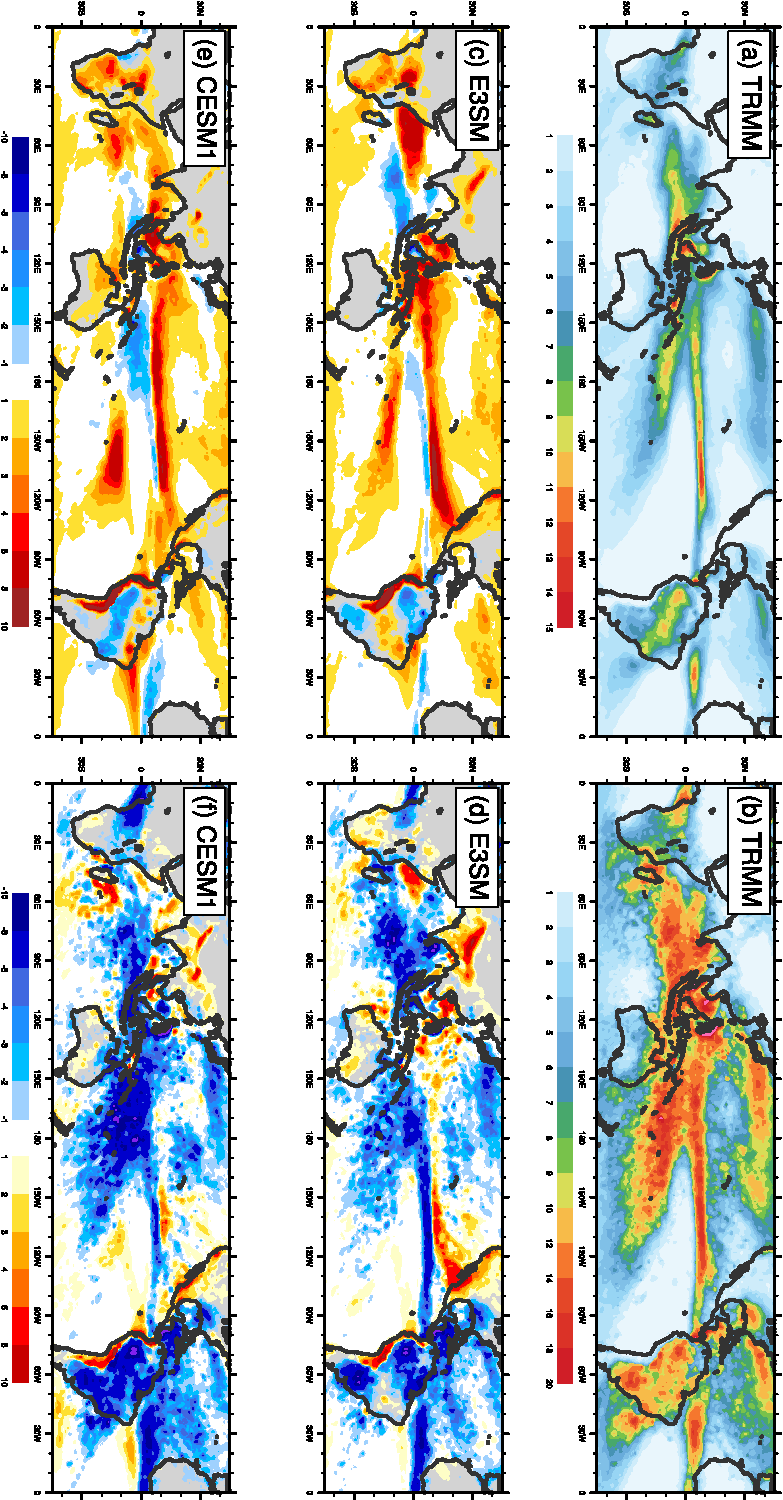
\includegraphics[width=0.5\textwidth,angle=90.]{./figs/f_mean_var_PRECT_DJF.pdf}
  \end{center}
  \caption{Observed TRMM Precipitation (1999-2013) for (a) mean and (b) standard deviation of daily amounts in mm/day. Difference from observations for E3SM (c) mean, (d) standard deviation and for CESM1 (e) mean and (f) standard deviation. Model average periods are for 15 years from CMIP5 and CMIP6 pre-industrial control experiments.} 
\label{f_mean_var_PRECT_DJF}
\end{figure}


\begin{figure}[fp]
  \begin{center}
    \noindent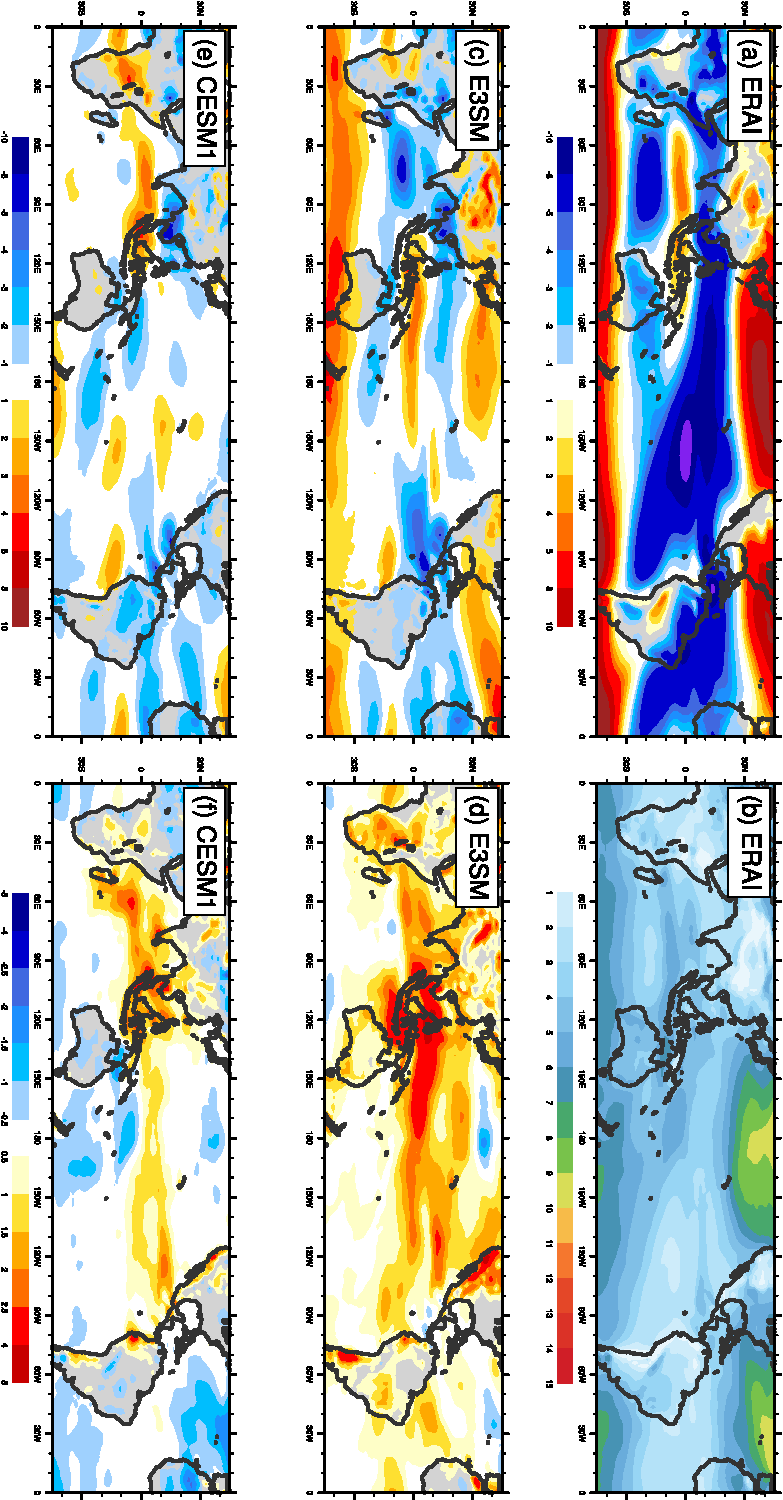
\includegraphics[width=0.5\textwidth,angle=90.]{./figs/f_mean_var_U850_DJF.pdf}
  \end{center}
  \caption{Observed ERA-interim 850-hPa zonal wind (1999-2013) for (a) mean and (b) standard deviation of daily amounts in mm/day. Difference from observations for E3SM (c) mean, (d) standard deviation and for CESM1 (e) mean and (f) standard deviation. Model average periods are for 15 years from CMIP5 and CMIP6 pre-industrial control experiments} 
\label{f_mean_var_U850_DJF}
\end{figure}

\
\begin{figure}[fp]
  \begin{center}
    \noindent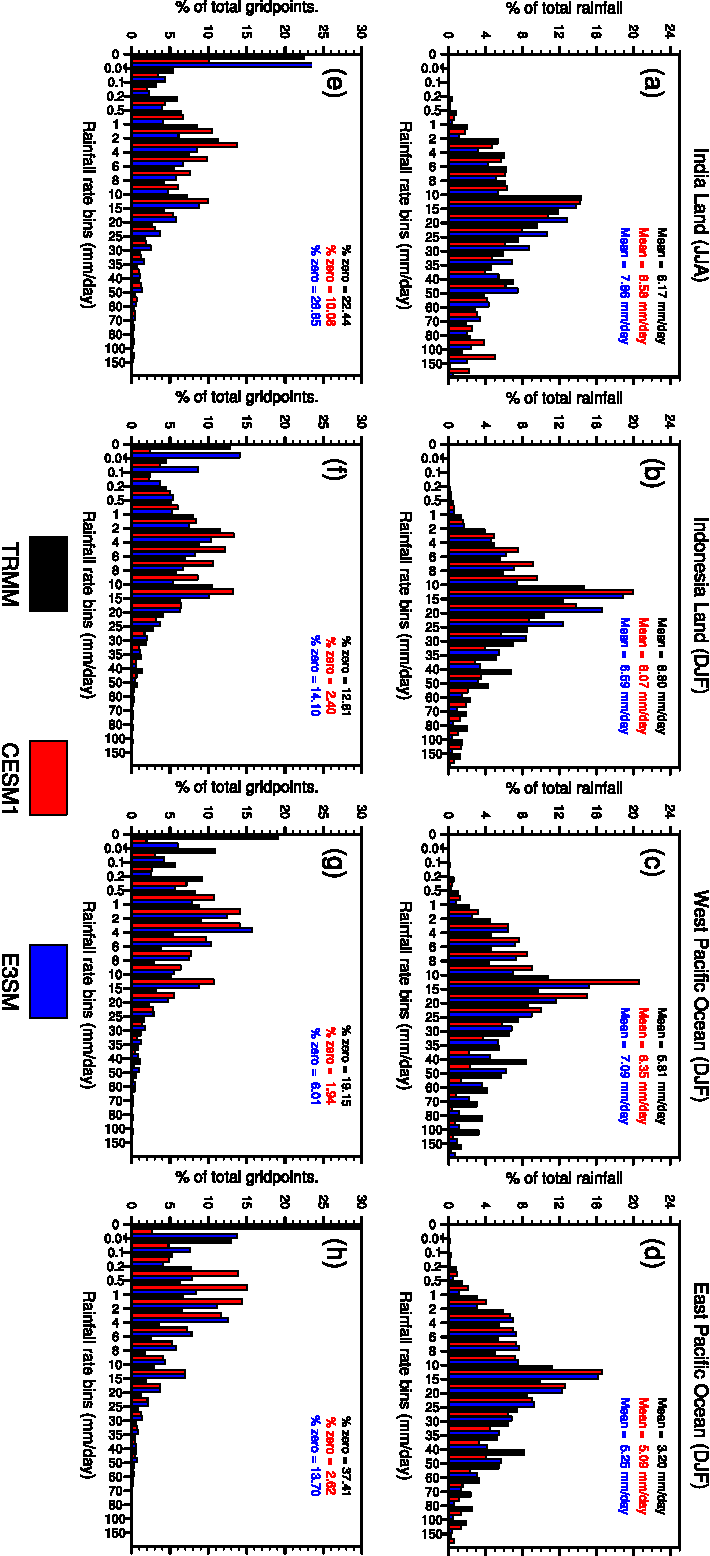
\includegraphics[width=0.6\textwidth,angle=90.]{./figs/f_pdf_PRECT.pdf}
  \end{center}
  \caption{Seasonal probability distributions of daily precipitation rate (mm/day) for 15 years over Indo-Pacific regions: Indian Ocean (a,d) [10\deg S-10\deg N, 60\deg E-95\deg E], Indonesia Land (b,e) [10\deg S-10\deg N, 100\deg E-150\deg E] and West Pacific Ocean (c,f) [20\deg S-0\deg N, 155E-180E] (a) through (c) is the percentage of total rainfall that each bin contributes. (d) through (f) is the percentage of the total number samples contributing to that rainfall rate. TRMM observations are interpolated to a 1\deg$ $ grid coincident with the E3SM grid.} 
\label{f_pdf_PRECT}
\end{figure}

\begin{figure}[fp]
  \begin{center}
    \noindent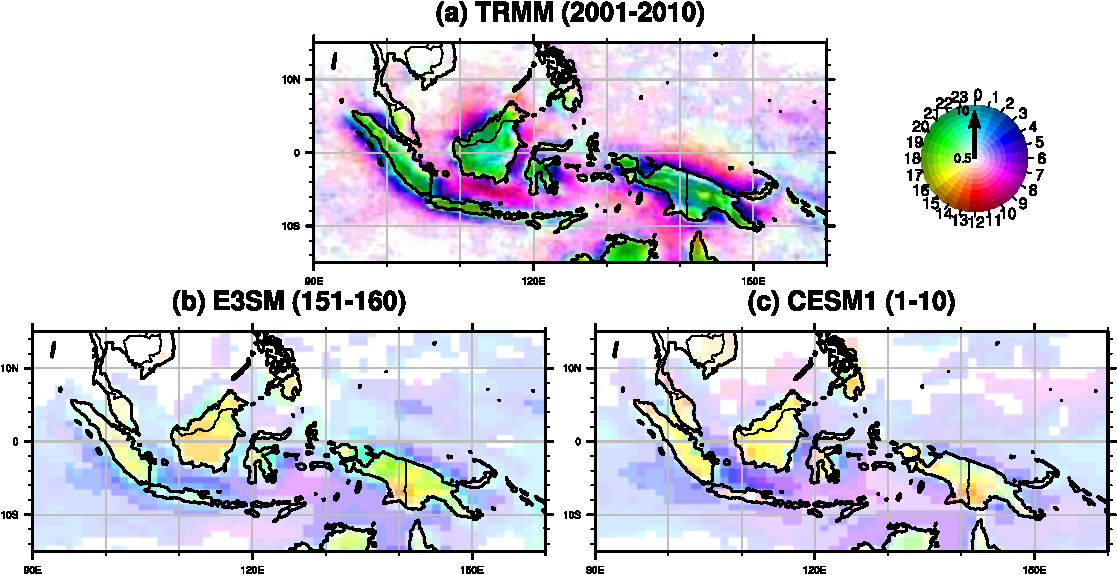
\includegraphics[width=0.9\textwidth,angle=0.]{./figs/f_dcycle_indo.pdf}
  \end{center}
  \caption{The diurnal cycle of precipitation (mm/day) over the Maritime Continent Region in DJF for (a) TRMM, (b) E3SM and (c) CESM1. Local diurnal timing (color hue) and magnitude (color saturation) are calculated based on 3-hourly data and averaged over 10 years.}
\label{f_dcycle_indo}
\end{figure}

\begin{figure}[t]
  \begin{center}
    \noindent 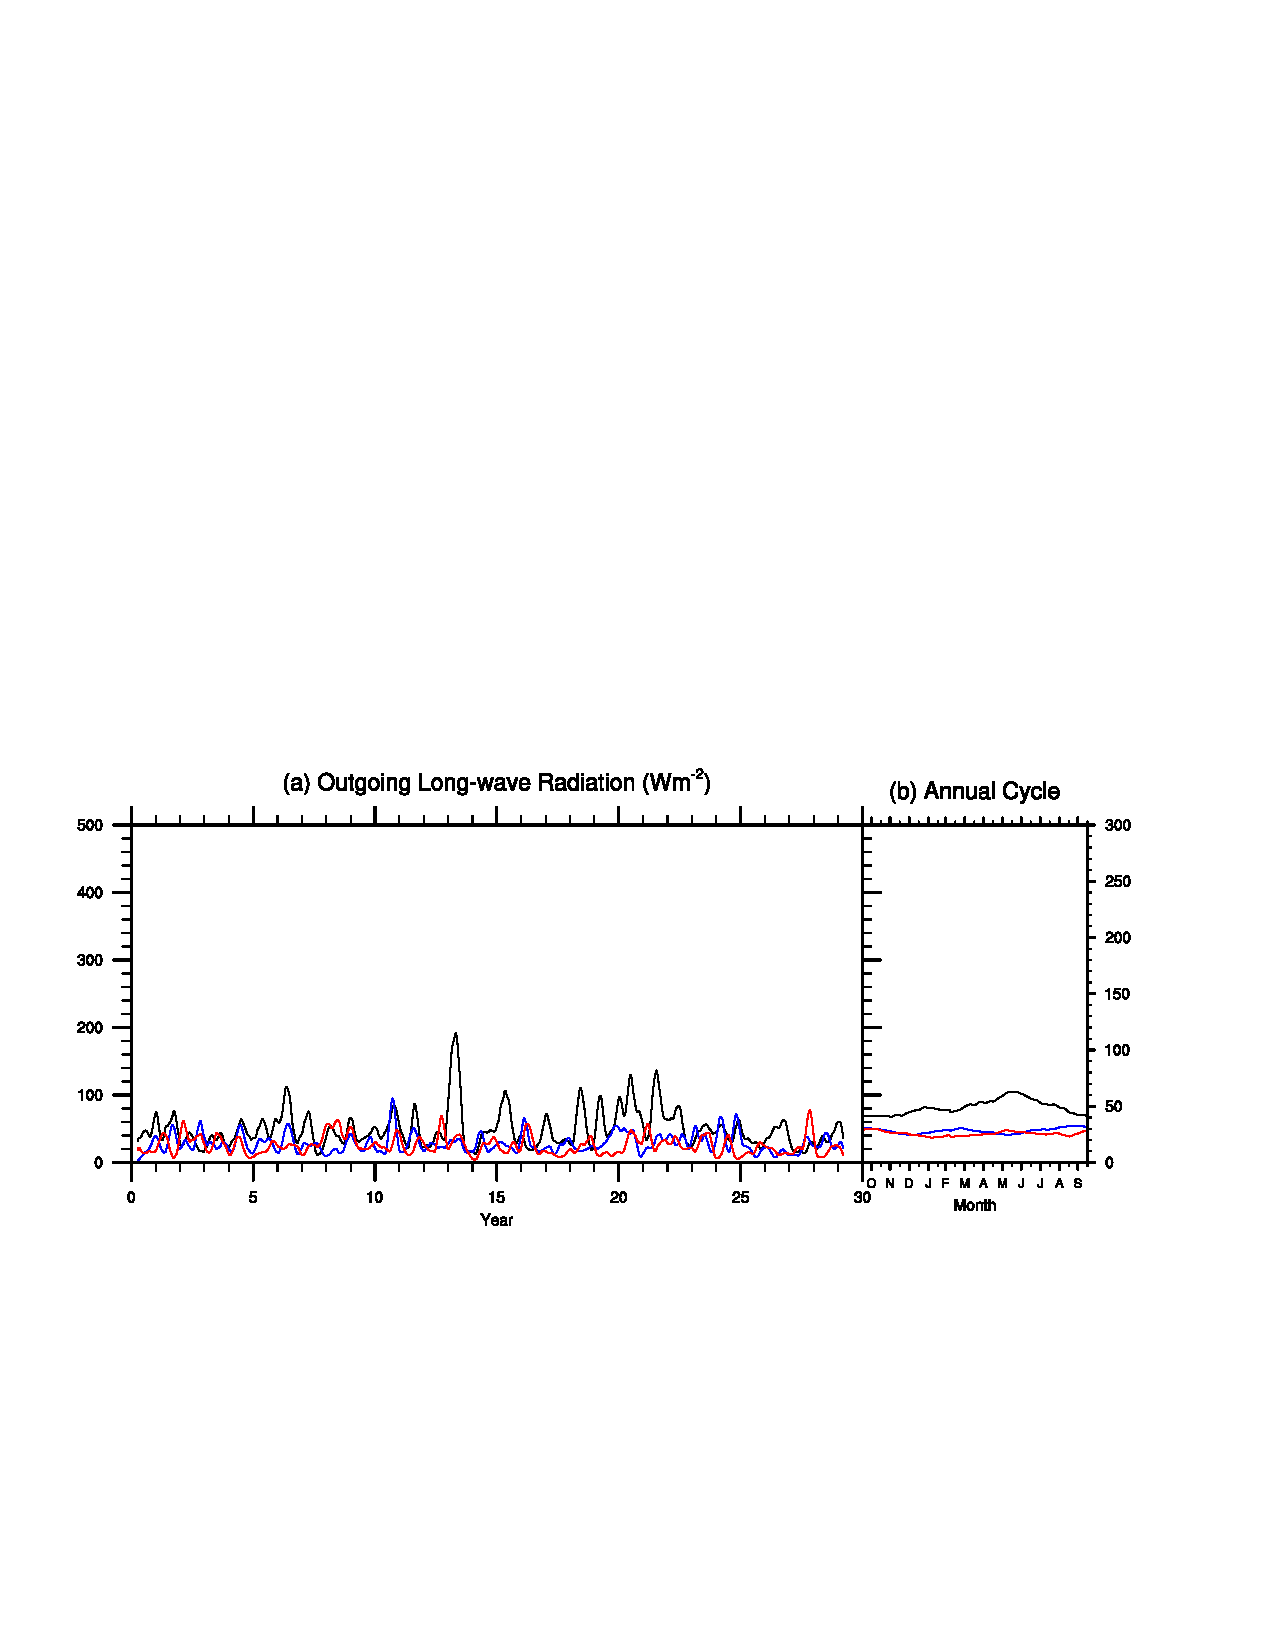
\includegraphics[width=1.1\textwidth,angle=0.] {./figs/f_bpass.pdf}
  \end{center}
  \caption{Band-pass (20-100 days) filtered, daily outgoing long-wave radiation Wm$^{-2}$ averaged in the Indo-Pacific region between 60\deg E and 180\deg E for 30-year segment of observed (NOAA: 1983-2004, black) and 30-year segments of the coupled models, CESM1 (red) and E3SM (blue).}
\label{f_bpass}
\end{figure}

\begin{figure}[t]
  \begin{center}
    \noindent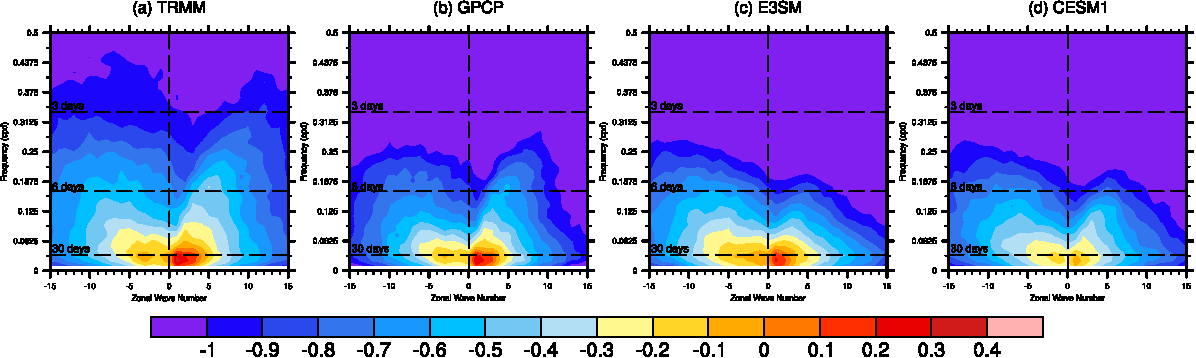
\includegraphics[width=1.1\textwidth,angle=0.]
    {./figs/f_kf_sym_PRECT.pdf}
  \end{center}
  \caption{Raw wavenumber-frequency power spectra \citep[following][]{Wheeler1999} of precipitation [ln(mm/day)], filtered over 20-100 day timescales, and only for propagating disturbances symmetric about the equator (15\deg S-15\deg N) from (a) TRMM, (b) GPCP, observations with (c) E3SM and (d) CESM1 from pre-industrial CMIP control simulations} 
\label{f_kf_sym_PRECT}
\end{figure}

\begin{figure}[fp]
  \begin{center}
    \noindent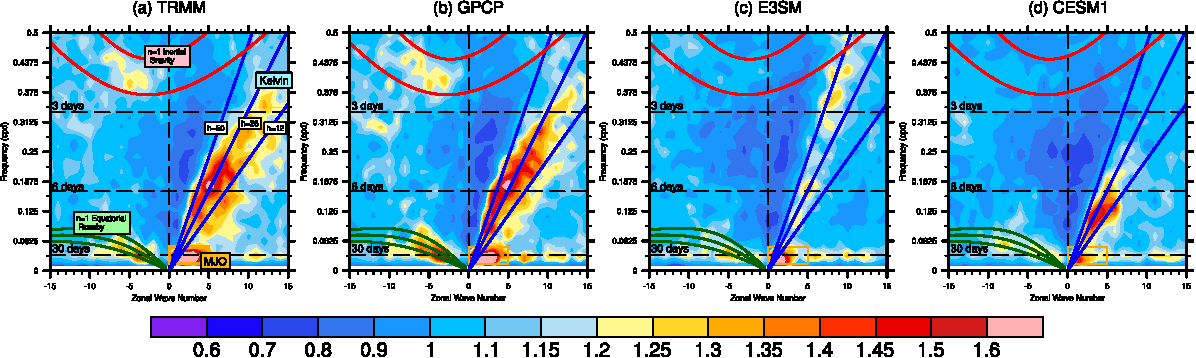
\includegraphics[width=1.1\textwidth,angle=0.]{./figs/f_kf_sym_ratio_PRECT.pdf}
  \end{center}
  \caption{Ratio of filtered wavenumber frequency power spectra for total precipitation, above a smoothed pseudo-red background spectra of the same field (15\deg S-15\deg N), for (a) TRMM, (b) GPCP, observations with (c) E3SM and (d) CESM1 from CMIP pre-industrial control simulations.} 
\label{f_kf_sym_ratio_PRECT}
\end{figure} 

\begin{figure}[t]
  \begin{center}
    \noindent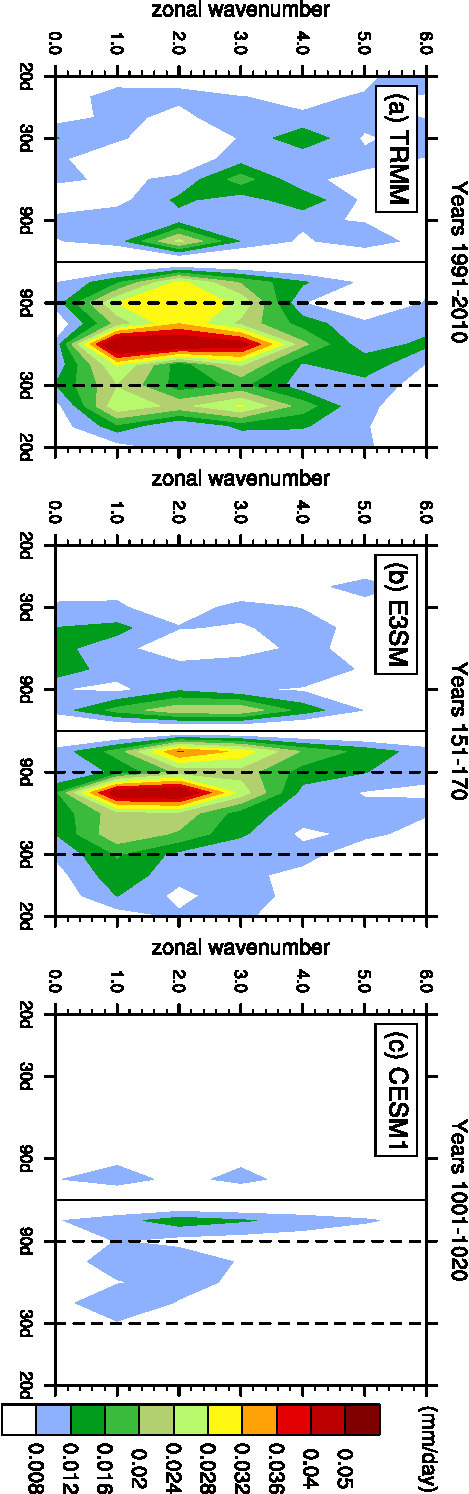
\includegraphics[width=0.3\textwidth,angle=90.]{./figs/f_mjo_spectra_PRECT_djf.pdf}
  \end{center}
  \caption{Wavenumber frequency spectrum focused on MJO sub-seasonal periods and frequencies for total precipitation (mm/day) from (a) TRMM, (b) E3SM and (c) CESM1.} 
\label{f_mjo_spectra_PRECT_djf}
\end{figure}

\begin{figure}[t]
  \begin{center}
    \noindent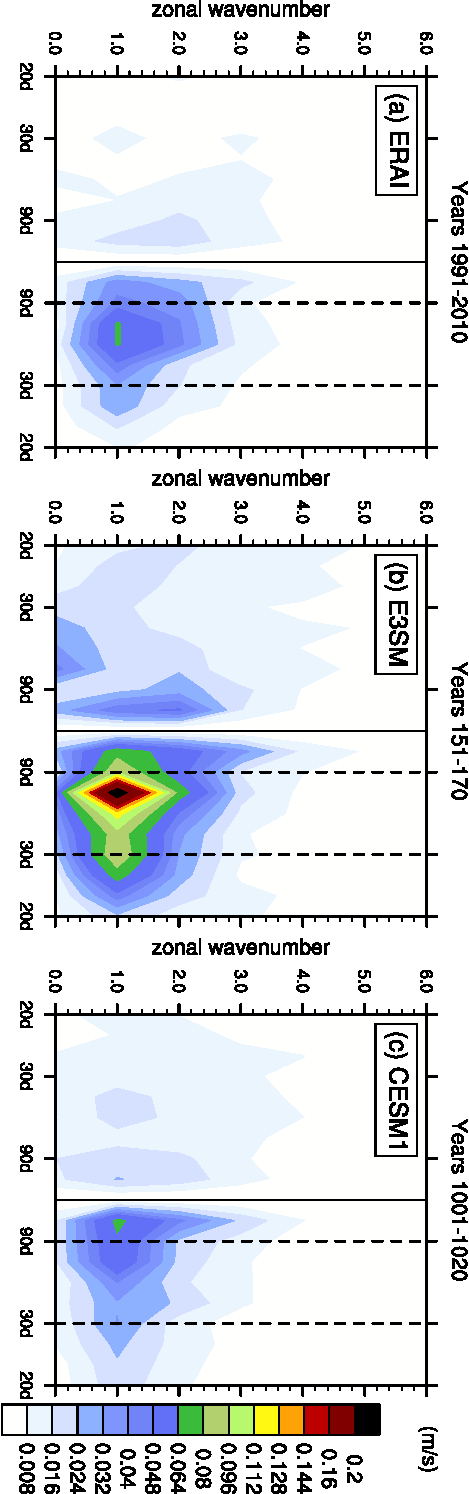
\includegraphics[width=0.3\textwidth,angle=90.]{./figs/f_mjo_spectra_U850_djf.pdf}
  \end{center}
  \caption{Wavenumber frequency spectrum focused on MJO sub-seasonal periods and frequencies for 850-hPa zonal wind (m/s) from (a) ERA-interim reanalysis, (b) E3SM and (c) CESM1.} 
\label{f_mjo_spectra_U850_djf}
\end{figure}

\begin{figure}[t]
  \begin{center}
    \noindent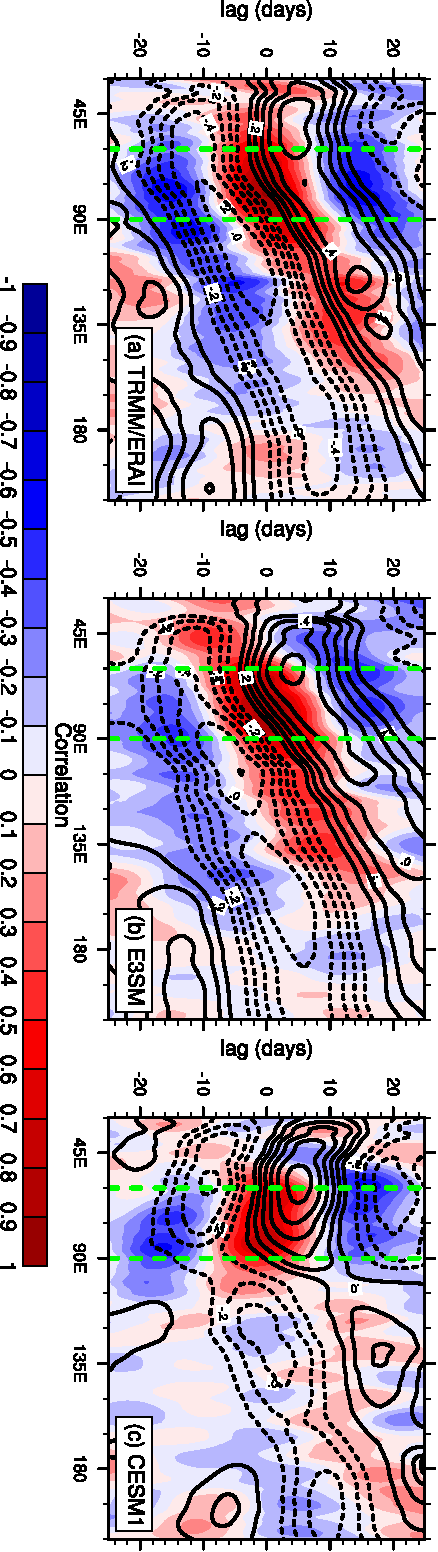
\includegraphics[width=0.3\textwidth,angle=90.]{./figs/f_lagcorr_djf.pdf}
  \end{center}
  \caption{The lag-correlation between DJF precipitation in the eastern Indian Ocean (60\deg E - 90\deg E) and precipitation (colors) and 850-hPa zonal wind (lines) at all other longitudes in the Indo-Pacific region for (a) TRMM and ERA-interim, (b) E3SM pre-industrial and (c) CESM1 pre-industrial forcing simulations (30 years). Band pass filtering (20-100 days) is applied to daily data averaged between 10\deg S - 10\deg N} 
\label{f_lagcorr_djf}
\end{figure}

\begin{figure}[t]
  \begin{center}
    \noindent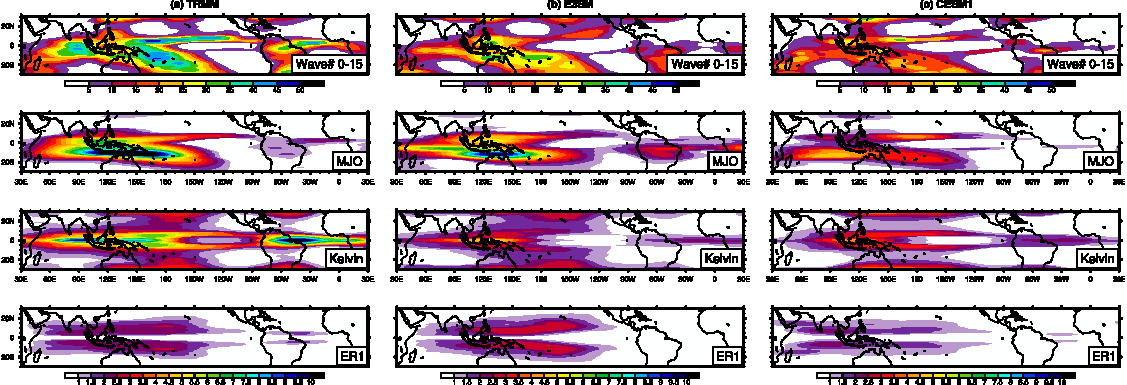
\includegraphics[width=1.1\textwidth,angle=0.]{./figs/f_wave_var_DJF_PRECT.pdf}
  \end{center}
  \caption{Regional variance of a inverse transformed daily precipitation field (mm/day)$^2$ after filtering for wavenumber frequency regions specific to wavenumbers -15 to +15 and for MJO, Kelvin and n=1 Rossby propagating modes of variability. Shown are (a) TRMM observations, with (b) E3SM and (c) CESM1 simulations} 
\label{f_wave_var_DJF_PRECT}
\end{figure}

\begin{figure}[t]
  \begin{center}
   \noindent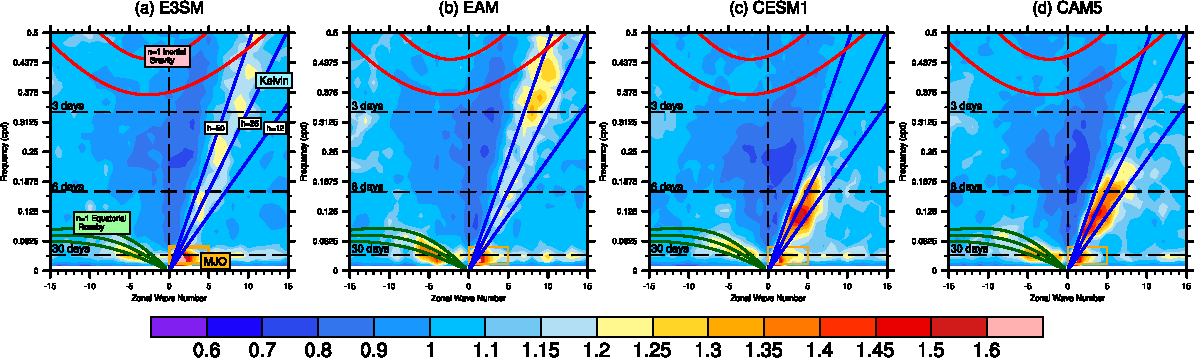
\includegraphics[width=1.0\textwidth,angle=0.]{./figs/f_eam_e3sm_kf.pdf}
  \end{center}
  \caption{Ratio of the wavenumber-frequency decomposition above a smooth background spectra of precipitation of historical simulations for E3SM (a) fully coupled and (b) EAM (AMIP) and CESM1 (c) fully coupled and (d) CAM5 (AMIP). Based on daily data averaged 15\deg S - 15\deg N.} 
\label{f_eam_e3sm_kf}
\end{figure}

\begin{figure}[t]
  \begin{center}
   \noindent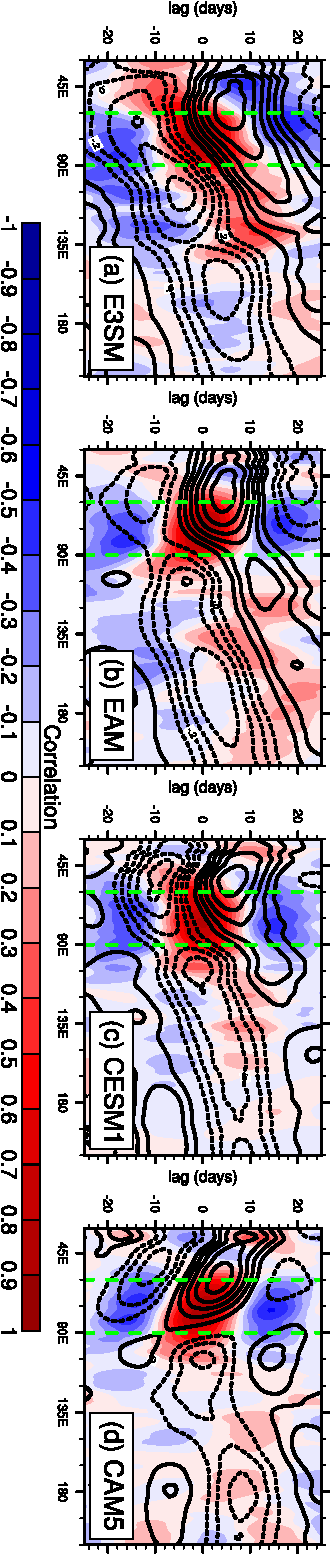
\includegraphics[width=0.21\textwidth,angle=90.]{./figs/f_eam_e3sm_lagcorr.pdf}
  \end{center}
  \caption{The lag-correlation between DJF precipitation in the eastern Indian Ocean (60\deg E - 90\deg E) and precipitation (colors) and 850-hPa zonal wind (lines) at all other longitudes in the Indo-Pacific region for (a) E3SM, (b) EAM (AMIP) (c) CESM1 and (d) CAM5 (AMIP) historical forcing simulations for 1986-2005. Band pass filtering (20-100 days) is applied to daily data averaged between 10\deg S - 10\deg N} 
\label{f_e3sm_lagcorr}
\end{figure}

\begin{figure}[t]
  \begin{center}
   \noindent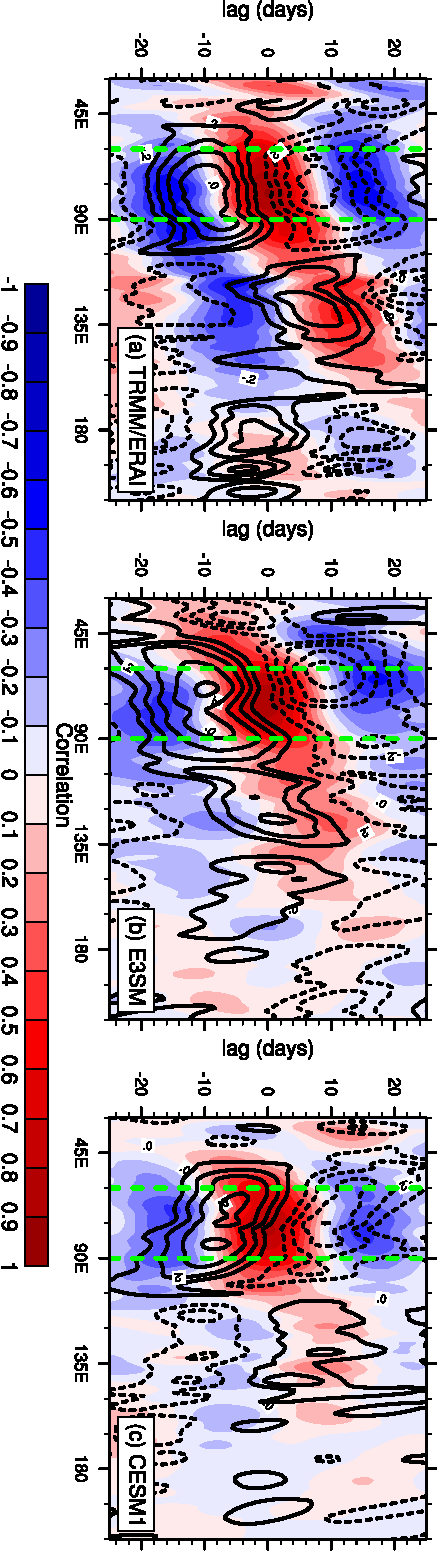
\includegraphics[width=0.3\textwidth,angle=90.]{./figs/f_lagcorr_ts_djf.pdf}
  \end{center}
  \caption{The lag-correlation between DJF precipitation in the eastern Indian Ocean (60\deg E - 90\deg E) and precipitation (colors) and surface temperature (lines) at all other longitudes in the Indo-Pacific region for (a) TRMM and ERAI, (b) E3SM and (c) CESM1 and pre-industrial forcing simulations for (30 years). Band pass filtering (20-100 days) is applied to daily data averaged between 10\deg S - 10\deg N.} 
\label{f_lagcorr_ts_djf}
\end{figure}

\begin{figure}[t]
  \begin{center}
   \noindent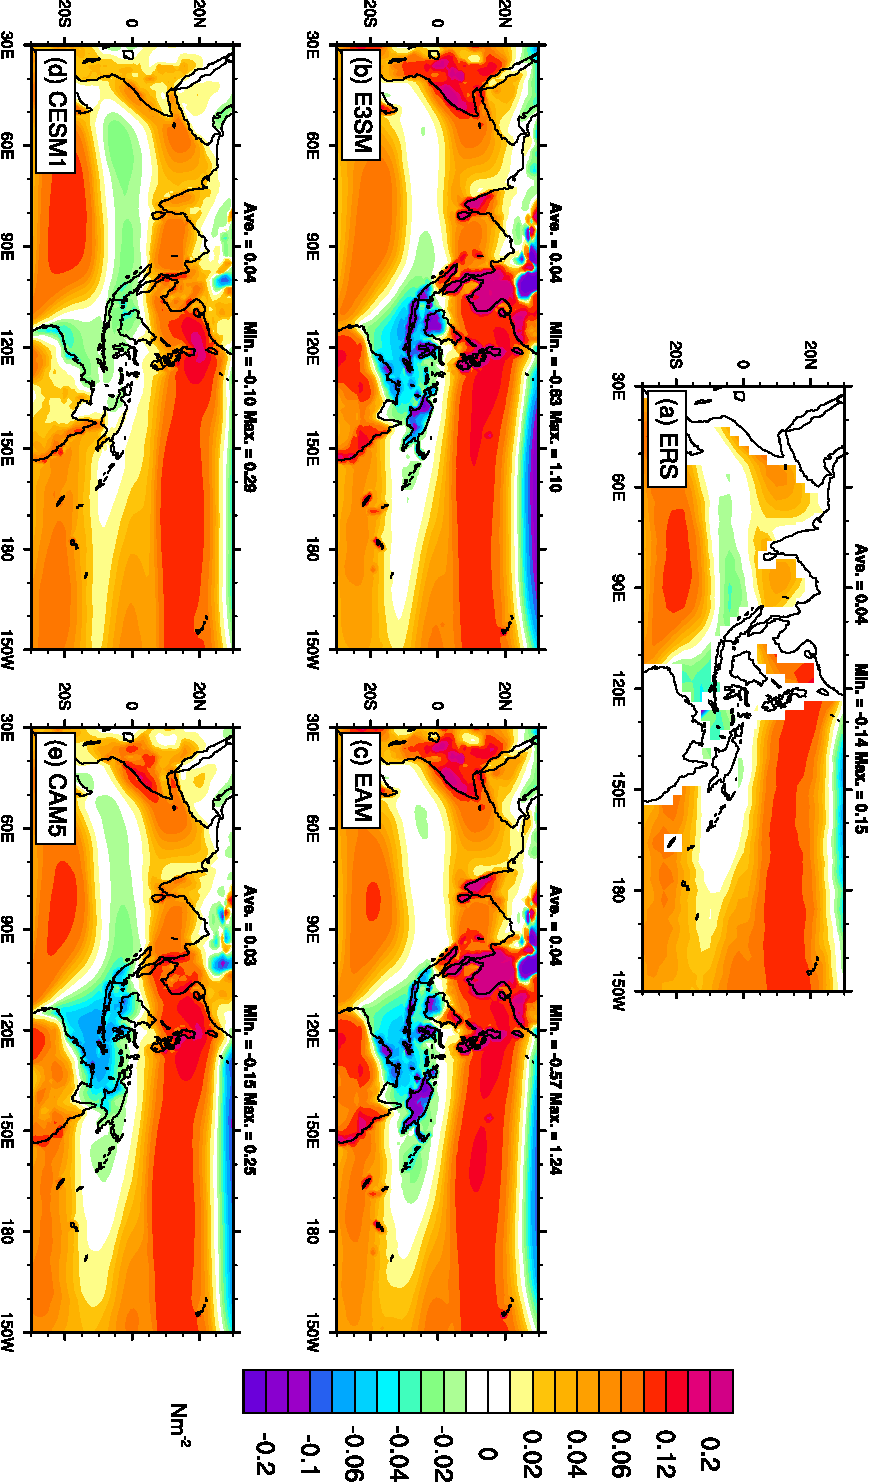
\includegraphics[width=0.6\textwidth,angle=90.]{./figs/f_E3SM_EAM_TAUX_DJF.pdf}
  \end{center}
  \caption{Surface zonal stress (Nm$^{-2}$) from observations (a) ERS, and model simulated equivalents for (b) E3SM, (c) EAM (AMIP), (d) CESM1 and (e) CAM5 (AMIP). Negative/positive values indicate westerly/easterly near surface winds.} 
\label{f_E3SM_EAM_TAUX_DJF}
\end{figure}

\begin{figure}[t]
  \begin{center}
   \noindent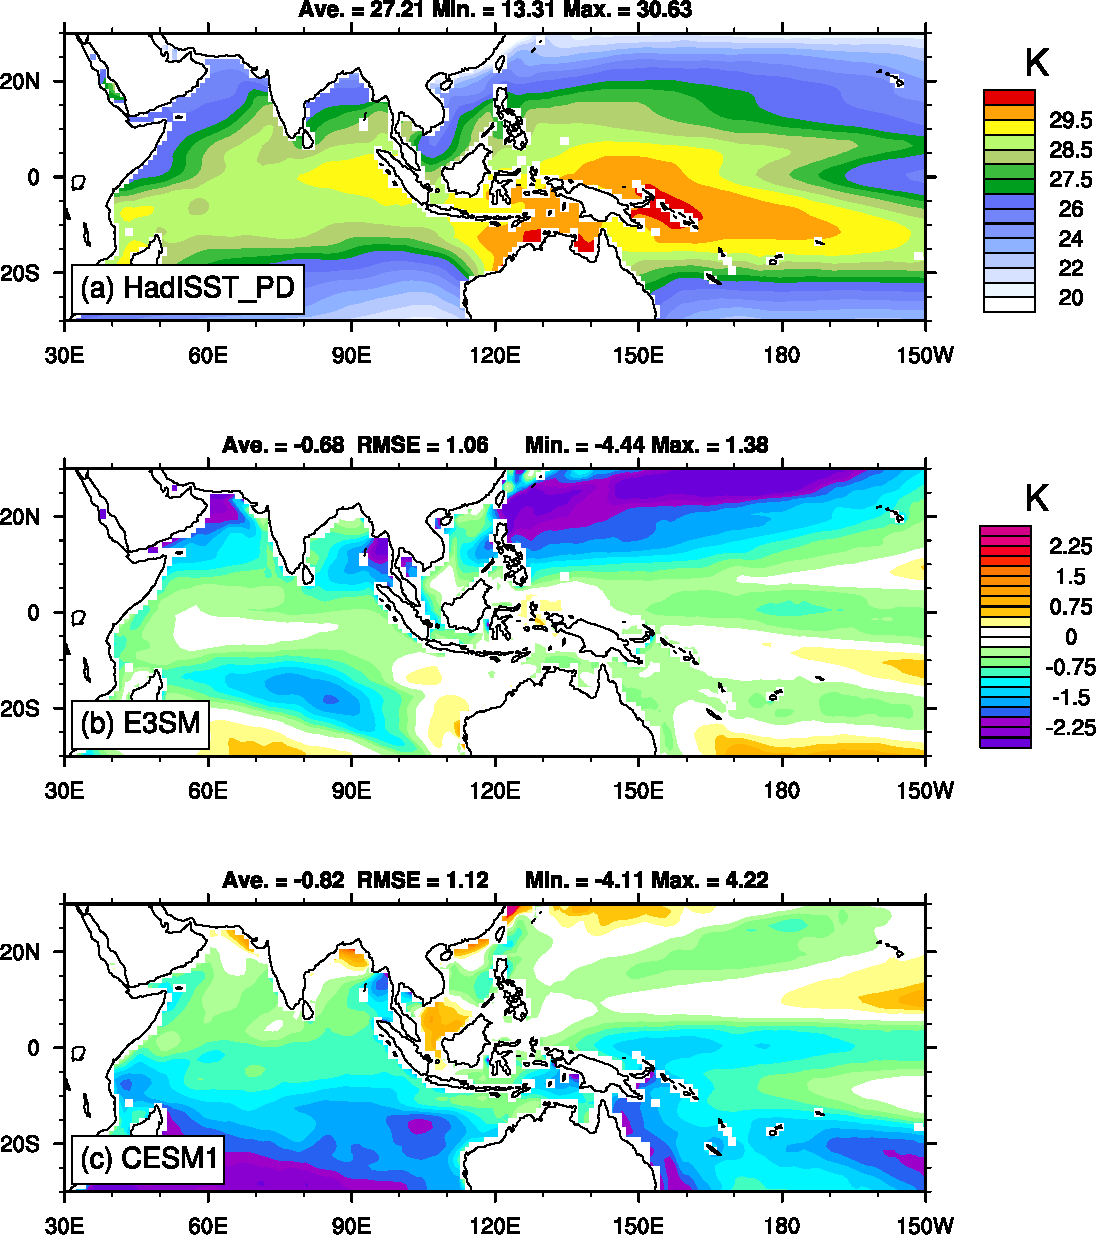
\includegraphics[width=0.8\textwidth]{./figs/f_E3SM_TS_DJF_diff.pdf}
  \end{center}
  \caption{Climatological Sea surface temperature distributions during DJF for (a) Observations \citep[HadISST,][]{Hurrell2008} (\deg C), and biases in (b) E3SM and (c) CESM1 of the present-day period (1986-2005) from 20th century historical simulations (\deg C).}
\label{f_E3SM_TS_DJF_diff}
\end{figure}



\begin{figure}[t]
  \begin{center}
   \noindent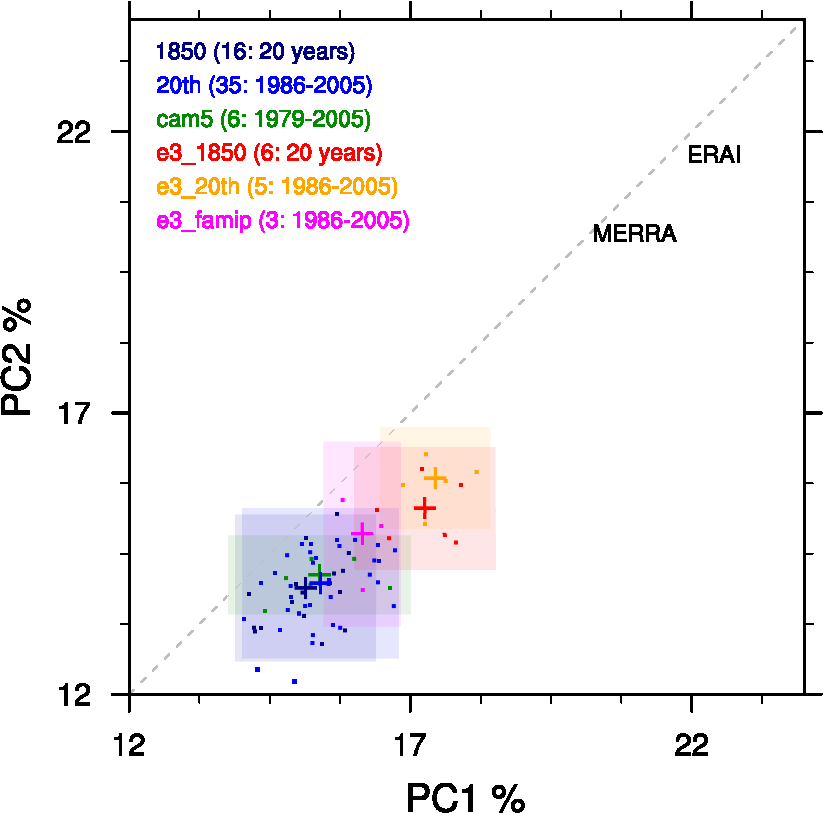
\includegraphics[width=0.8\textwidth]{./figs/f_pc1pc2.pdf}
  \end{center}
  \caption{The sub-seasonal (20-100 day) variance described by principle components 1 and 2 of the multivariate combined EOFs of Outgoing Longwave Radiation, 850-hPa zonal wind and 200-hPa. Colors and dots denote ensembles for different model variations with EAM (e3\_famip)/CAM5 (cam5) as present-day AMIP, E3SM (e3\_1850)/CESM1 (1850) as pre-industrial (1850 control) and present-day E3SM (e3\_20th)/CESM1 (20th) CMIP5 scenarios . Shading indicates +/- 2 standard deviations across both PC1 and PC2 axes.} 
\label{f_e3sm_pc1pc2}
\end{figure}

\begin{figure}[t]
  \begin{center}
  \noindent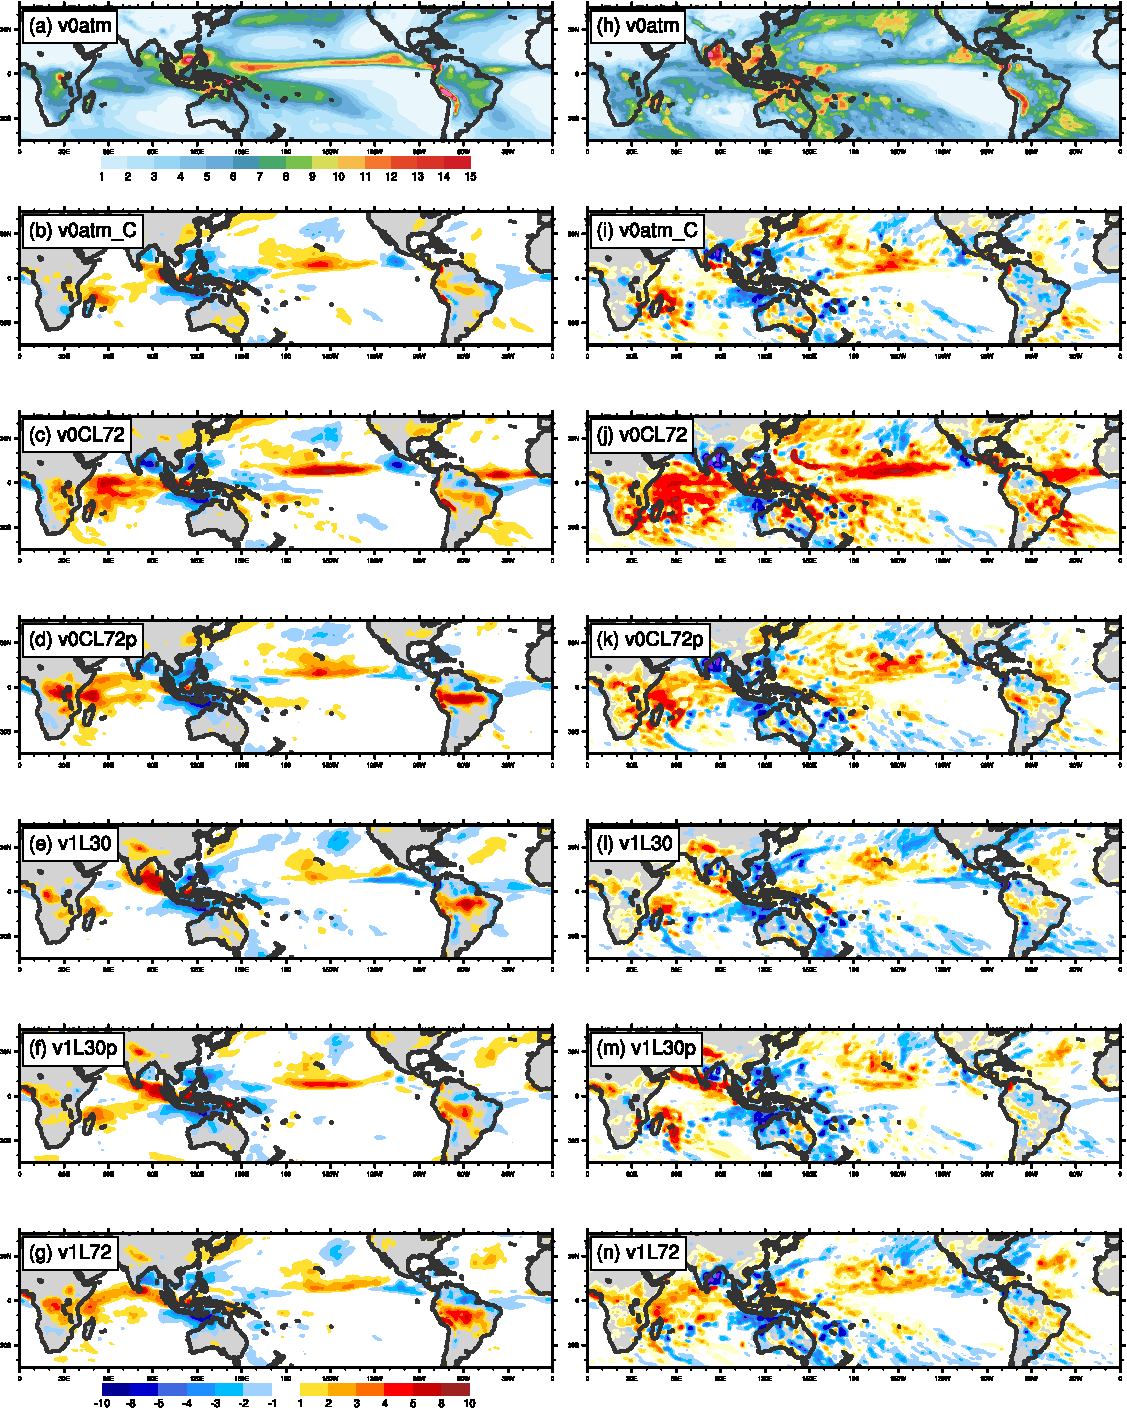
\includegraphics[width=0.9\textwidth,angle=0.]{./figs/f_sens_stats_PRECT_djf}
  \caption{\small{Precipitation mean (left panels) and variance (right panels) from the 2000 climatology control AMIP-type sensitivity experiments for (a) v0atm control (EAMv0, same as CAM5.3 physics), and differences from the control of the sensitivity experiments: (b,i) control with CLUBB and MG2 added (v0atm\_C); (c,j) as v0CL72, but with 72 vertical levels (v0CL72); (d,k) as v0CL72, but with climate retuning parameters from v1L72/EAMv1; (e,l) final EAMv1 tunings, but with 30 vertical levels (v1L30); (f,m) retuning of v1L30 for climate  (g,n) final version of EAMv1 (v1L72). All simulations use the modified CAM5 deep convection settings of lifting level (2) and (stable layers allowed, capeten=1) apart from v0atm, v0atm\_C and which use the previous default settings (capeten=5, lifting level=0). For an expanded description of the experiment configurations see table \ref{tab:sens_sims} or table 1 of \cite{Xie2018}.}} 
  \end{center}
\label{f_sens_stats_PRECT_djf}
\end{figure}

\begin{figure}[t]
  \begin{center}
  \noindent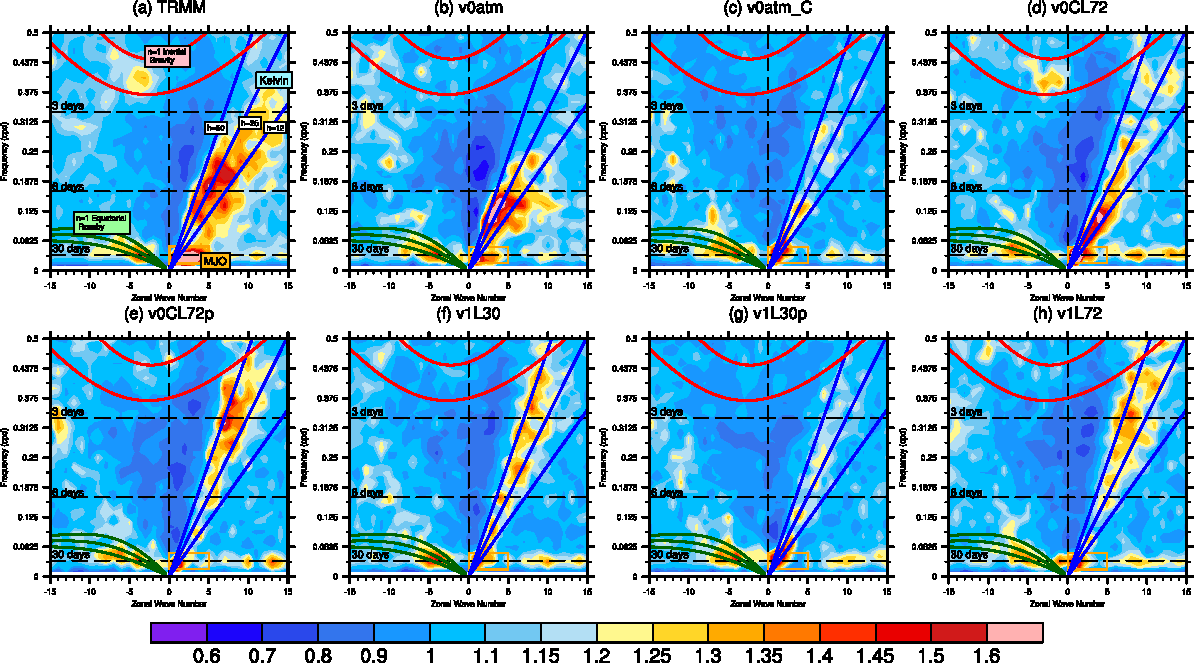
\includegraphics[width=0.9\textwidth,angle=0.]{./figs/f_sens_kf.pdf}
  \caption{Wavenumber frequency decomposition of total precipitation as described in Figure \ref{f_kf_sym_ratio_PRECT} for (a) observations (TRMM) and for the EAM configuration sensitivity experiments (b) v0atm, (c) v0atm\_C, (d) v0atm\_C, (e) v0CL72p, (f) v1L30, (g) v1L30p and (h) v1L72. Experiments are described in Figure \ref{f_sens_stats_PRECT_djf}. } 
  \end{center}
\label{f_sens_kf}
\end{figure}

\begin{figure}[t]
  \begin{center}
  \noindent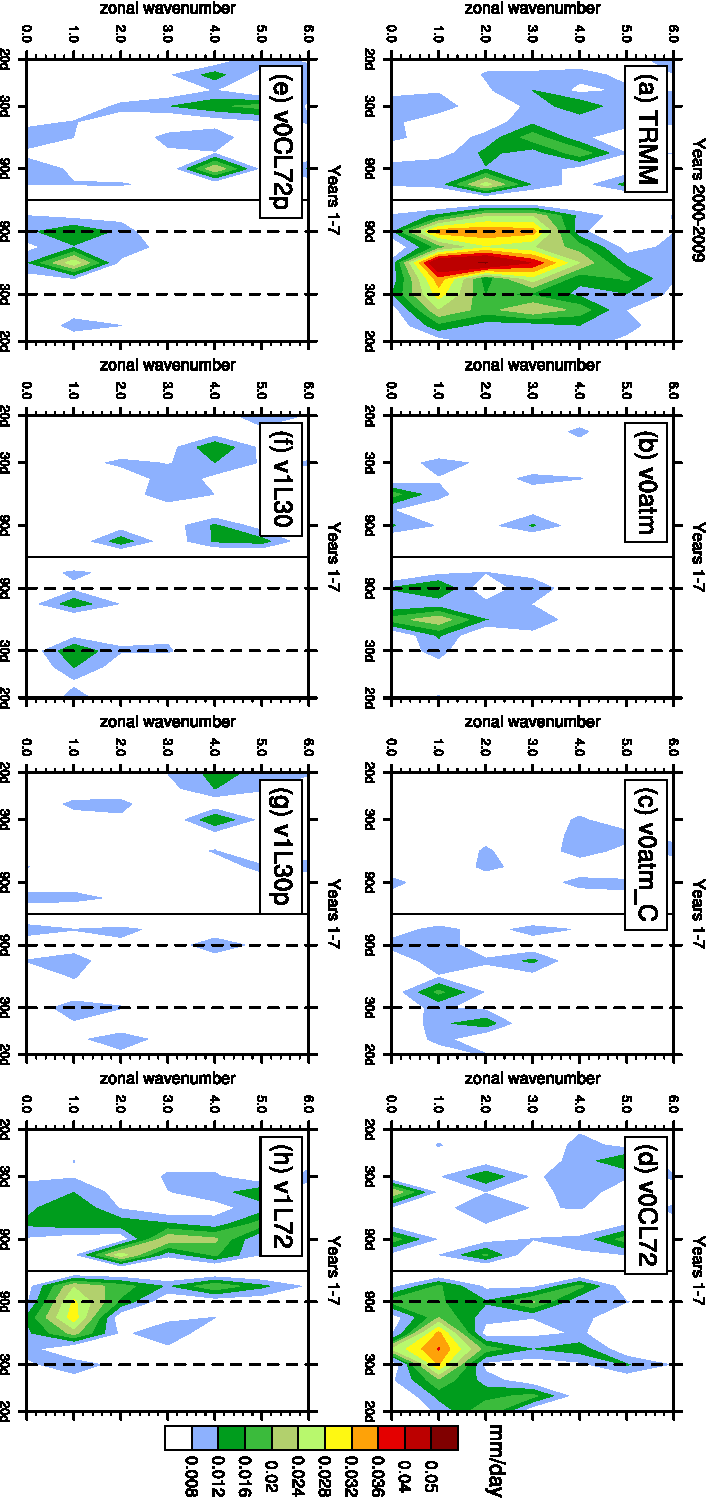
\includegraphics[width=0.45\textwidth,angle=90.]{./figs/f_sens_spectra.pdf}
  \caption{Wavenumber frequency decomposition of total precipitation as described in Figure \ref{f_kf_sym_ratio_PRECT} for (a) observations (TRMM) and for the EAM configuration sensitivity experiments (b) v0at,m, v0atm\_C, (c) v0CL72, (d) v0CL72p, (e) v0CL72p, (f) v0L30, (g) v1L30p and (h) v1L72. Experiments are described in Figure \ref{f_sens_stats_PRECT_djf}. } 
  \end{center}
\label{f_sens_spectra}
\end{figure}

\newpage

%Run BiBTeX on your LaTeX
% file.
%
% 3. Open the new .bbl file containing the reference list and
%   copy all the contents into your LaTeX file here.
%
% 4. Comment out the old \bibliographystyle and \bibliography commands.
%
% 5. Run LaTeX on your new file before submitting.
%
% AGU does not want a .bib or a .bbl file. Please copy in the contents of your .bbl file here.

%\begin{thebibliography}{}

%\providecommand{\natexlab}[1]{#1}
%\expandafter\ifx\csname urlstyle\endcsname\relax
%  \providecommand{\doi}[1]{doi:\discretionary{}{}{}#1}\else
%  \providecommand{\doi}{doi:\discretionary{}{}{}\begingroup
%  \urlstyle{rm}\Url}\fi
%
%\bibitem[{\textit{Atkinson and Sloan}(1991)}]{AtkinsonSloan}
%Atkinson, K., and I.~Sloan (1991), The numerical solution of first-kind
%  logarithmic-kernel integral equations on smooth open arcs, \textit{Math.
%  Comp.}, \textit{56}(193), 119--139.
%
%\bibitem[{\textit{Colton and Kress}(1983)}]{ColtonKress1}
%Colton, D., and R.~Kress (1983), \textit{Integral Equation Methods in
%  Scattering Theory}, John Wiley, New York.
%
%\bibitem[{\textit{Hsiao et~al.}(1991)\textit{Hsiao, Stephan, and
%  Wendland}}]{StephanHsiao}
%Hsiao, G.~C., E.~P. Stephan, and W.~L. Wendland (1991), On the {D}irichlet
%  problem in elasticity for a domain exterior to an arc, \textit{J. Comput.
%  Appl. Math.}, \textit{34}(1), 1--19.
%
%\bibitem[{\textit{Lu and Ando}(2012)}]{LuAndo}
%Lu, P., and M.~Ando (2012), Difference of scattering geometrical optics
%  components and line integrals of currents in modified edge representation,
%  \textit{Radio Sci.}, \textit{47},  RS3007, \doi{10.1029/2011RS004899}.

%\end{thebibliography}

%Reference citation examples:

%...as shown by \textit{Kilby} [2008].
%...as shown by {\textit  {Lewin}} [1976], {\textit  {Carson}} [1986], {\textit  {Bartholdy and Billi}} [2002], and {\textit  {Rinaldi}} [2003].
%...has been shown [\textit{Kilby et al.}, 2008].
%...has been shown [{\textit  {Lewin}}, 1976; {\textit  {Carson}}, 1986; {\textit  {Bartholdy and Billi}}, 2002; {\textit  {Rinaldi}}, 2003].
%...has been shown [e.g., {\textit  {Lewin}}, 1976; {\textit  {Carson}}, 1986; {\textit  {Bartholdy and Billi}}, 2002; {\textit  {Rinaldi}}, 2003].

%...as shown by \citet{jskilby}.
%...as shown by \citet{lewin76}, \citet{carson86}, \citet{bartoldy02}, and \citet{rinaldi03}.
%...has been shown \citep{jskilbye}.
%...has been shown \citep{lewin76,carson86,bartoldy02,rinaldi03}.
%...has been shown \citep [e.g.,][]{lewin76,carson86,bartoldy02,rinaldi03}.
%
% Please use ONLY \citet and \citep for reference citations.
% DO NOT use other cite commands (e.g., \cite, \citeyear, \nocite, \citealp, etc.).

%% ------------------------------------------------------------------------ %%
%
%  END ARTICLE
%
%% ------------------------------------------------------------------------ %%






\end{article}







%
%
%% Enter Figures and Tables here:
%
% DO NOT USE \psfrag or \subfigure commands.
%
% Figure captions go below the figure.
% Table titles go above tables; all other caption information
%  should be placed in footnotes below the table.
%
%----------------
% EXAMPLE FIGURE
%
% \begin{figure}
% \noindent\includegraphics[width=20pc]{samplefigure.eps}
% \caption{Caption text here}
% \label{figure_label}
% \end{figure}






%
% ---------------
% EXAMPLE TABLE
%
%\begin{table}
%\caption{Time of the Transition Between Phase 1 and Phase 2\tablenotemark{a}}
%\centering
%\begin{tabular}{l c}
%\hline
% Run  & Time (min)  \\
%\hline
%  $l1$  & 260   \\
%  $l2$  & 300   \\
%  $l3$  & 340   \\
%  $h1$  & 270   \\
%  $h2$  & 250   \\
%  $h3$  & 380   \\
%  $r1$  & 370   \\
%  $r2$  & 390   \\
%\hline
%\end{tabular}
%\tablenotetext{a}{Footnote text here.}
%\end{table}

% See below for how to make sideways figures or tables.

\end{document}

%%%%%%%%%%%%%%%%%%%%%%%%%%%%%%%%%%%%%%%%%%%%%%%%%%%%%%%%%%%%%%%

%%More Information and Advice:

%% ------------------------------------------------------------------------ %%
%
%  SECTION HEADS
%
%% ------------------------------------------------------------------------ %%

% Capitalize the first letter of each word (except for
% prepositions, conjunctions, and articles that are
% three or fewer letters).

% AGU follows standard outline style; therefore, there cannot be a section 1 without
% a section 2, or a section 2.3.1 without a section 2.3.2.
% Please make sure your section numbers are balanced.
% ---------------
% Level 1 head
%
% Use the \section{} command to identify level 1 heads;
% type the appropriate head wording between the curly
% brackets, as shown below.
%
%An example:
%\section{Level 1 Head: Introduction}
%
% ---------------
% Level 2 head
%
% Use the \subsection{} command to identify level 2 heads.
%An example:
%\subsection{Level 2 Head}
%
% ---------------
% Level 3 head
%
% Use the \subsubsection{} command to identify level 3 heads
%An example:
%\subsubsection{Level 3 Head}
%
%---------------
% Level 4 head
%
% Use the \subsubsubsection{} command to identify level 3 heads
% An example:
%\subsubsubsection{Level 4 Head} An example.
%
%% ------------------------------------------------------------------------ %%
%
%  IN-TEXT LISTS
%
%% ------------------------------------------------------------------------ %%
%
% Do not use bulleted lists; enumerated lists are okay.
% \begin{enumerate}
% \item
% \item
% \item
% \end{enumerate}
%
%% ------------------------------------------------------------------------ %%
%
%  EQUATIONS
%
%% ------------------------------------------------------------------------ %%

% Single-line equations are centered.
% Equation arrays will appear left-aligned.

Math coded inside display math mode \[ ...\]
 will not be numbered, e.g.,:
 \[ x^2=y^2 + z^2\]

 Math coded inside \begin{equation} and \end{equation} will
 be automatically numbered, e.g.,:
 \begin{equation}
 x^2=y^2 + z^2
 \end{equation}

% IF YOU HAVE MULTI-LINE EQUATIONS, PLEASE
% BREAK THE EQUATIONS INTO TWO OR MORE LINES
% OF SINGLE COLUMN WIDTH (20 pc, 8.3 cm)
% using double backslashes (\\).

% To create multiline equations, use the
% \begin{eqnarray} and \end{eqnarray} environment
% as demonstrated below.
\begin{eqnarray}
  x_{1} & = & (x - x_{0}) \cos \Theta \nonumber \\
        && + (y - y_{0}) \sin \Theta  \nonumber \\
  y_{1} & = & -(x - x_{0}) \sin \Theta \nonumber \\
        && + (y - y_{0}) \cos \Theta.
\end{eqnarray}

%If you don't want an equation number, use the star form:
%\begin{eqnarray*}...\end{eqnarray*}

% Break each line at a sign of operation
% (+, -, etc.) if possible, with the sign of operation
% on the new line.

% Indent second and subsequent lines to align with
% the first character following the equal sign on the
% first line.

% Use an \hspace{} command to insert horizontal space
% into your equation if necessary. Place an appropriate
% unit of measure between the curly braces, e.g.
% \hspace{1in}; you may have to experiment to achieve
% the correct amount of space.


%% ------------------------------------------------------------------------ %%
%
%  EQUATION NUMBERING: COUNTERci
%
%% ------------------------------------------------------------------------ %%

% You may change equation numbering by resetting
% the equation counter or by explicitly numbering
% an equation.

% To explicitly number an equation, type \eqnum{}
% (with the desired number between the brackets)
% after the \begin{equation} or \begin{eqnarray}
% command.  The \eqnum{} command will affect only
% the equation it appears with; LaTeX will number
% any equations appearing later in the manuscript
% according to the equation counter.
%

% If you have a multiline equation that needs only
% one equation number, use a \nonumber command in
% front of the double backslashes (\\) as shown in
% the multiline equation above.

%% ------------------------------------------------------------------------ %%
%
%  SIDEWAYS FIGURE AND TABLE EXAMPLES
%
%% ------------------------------------------------------------------------ %%
%
% For tables and figures, add \usepackage{rotating} to the paper and add the rotating.sty file to the folder.
% AGU prefers the use of {sidewaystable} over {landscapetable} as it causes fewer problems.
%
% \begin{sidewaysfigure}
% \includegraphics[width=20pc]{samplefigure.eps}
% \caption{caption here}
% \label{label_here}
% \end{sidewaysfigure}
%
%
%
% \begin{sidewaystable}
% \caption{}
% \begin{tabular}
% Table layout here.
% \end{tabular}
% \end{sidewaystable}
%
%

